\documentclass[uplatex,a4paper,12pt,onecolumn,oneside,openany]{jsbook}


% 設定ファイル
\usepackage{mystyle}

\title{
{\Large 令和元年度 修士論文} \\[4cm]
\LARGE KinectとOpenCVを用いた
     \\参加型プロジェクションマッピングの試作 \\[4cm]
}
\author{宮崎大学 大学院 工学研究科修士課程\\
工学専攻 機械・情報系コース\\
T1803016 篠田貴大\\
\\
指導教員 坂本眞人 准教授
}
\date{令和2年1月27日}

\begin{document}
\maketitle

\clearpage

%%% 概要 %%%
\renewcommand{\thepage}{\roman{page}}
\renewcommand{\thepage}{\roman{page}}
\chapter*{概要}

近年,エンターテインメントコンピューティングが日本でますます注目されている.
その中でも本研究では,プロジェクションマッピングに着目した.
プロジェクションマッピングは,プロジェクターを使用して空間と映像を合成することにより、
新しい空間を作成する技術である。
多くの人がダンサーのパフォーマンスとプロジェクションマッピングが融合した作品に魅了されたことがあるだろう.
ただし、これらの作業では、パフォーマーがプロジェクションマッピングの画像オブジェクトの座標に
正確に動きを合わせる必要があるため多くの人にとって困難であると考える.

そこで,プロジェクションマッピングを見る人々だけでなく,パフォーマーも楽しませるために,
パフォーマーの動きに応じてインタラクティブに変化する参加型のプロジェクションマッピングを提案する.

本研究では,スポーツに焦点を当てKinectを用いて
野球のピッチングとサッカーのリフティング動作を行えるプロジェクションマッピングを実装した.
また,ユーザがKinectの視野から隠れた後,再度Kinectの視野内に
入った場合,ユーザの骨格座標の再追従が上手く行われない時がある問題に対しては
カスケード分類器を用いてユーザの検出を行う手法でアプローチした.

本研究で提案したプロジェクションマッピングに対する評価を得るために
X人の被験者に対してアンケーの実施を行った.

評価結果をかく

今後の課題としては,



%%% 目次 %%%

{\makeatletter
\let\ps@jpl@in\ps@empty
\makeatother
\pagestyle{plain}

\tableofcontents
\listoffigures
\listoftables
\pagestyle{fancy}
\clearpage}


%%%%%% 1. はじめに %%%%%%
\chapter{はじめに}
\thispagestyle{fancy}
\setcounter{page}{1}
\renewcommand{\thepage}{\arabic{page}}

\section{研究背景}
近年,エンターテインメントコンピューティングがますます注目され,日本の主要産業の1つとなった.

従来の工学は物質的な豊さを求められてきたが,それが飽和しつつある昨今,
精神的な豊さを求めるため新しいエンターテインメントを創造するための
技術とコンテンツの研究を行う研究分野がエンターテインメントコンピューティングである.
その中でも本研究では,プロジェクションマッピングに着目した.

プロジェクションマッピングは,プロジェクターを使用して空間と映像を合成することにより、
新しい空間を作成する技術である。
多くの人がダンサーのパフォーマンスとプロジェクションマッピングを組み合わせた素晴らしい
世界を作り出す作品に魅了されたことがあるだろう.
ただし、これらの作業では、パフォーマーがプロジェクションマッピングの画像オブジェクトの座標に
正確に動きを合わせる必要があるが、これは多くの人にとって困難であると考える.

本研究では、プロジェクションマッピングを見る人々だけでなく,パフォーマーも楽しませるために,
パフォーマーの動きに応じてインタラクティブに変化する参加型のプロジェクションマッピングを提案する.

\clearpage

\section{プロジェクションマッピングの歴史}
プロジェクションマッピングは最新の技術と思う人も多いだろうがそうでは無い.
ベースにある考え方や手法は実は古くから様々な場所で行われていた.
プロジェクターが様々なクリエイターの手に渡った時から,それを使った新たな表現を求め,
その流れの中で15年以上前から自然発生的に生まれてきた.特に舞台やイベント,
ビデオアートやインスタレーションといわれる表現の世界では早くから取り組まれ,
メディアアートとしても試行錯誤が行われている.

注目を集めるようになった理由として,まず機材や映像技術の発達である.
特に高輝度のプロジェクターがクリエイターの手に届くようになり,
ヨーロッパで建築物への大規模なプロジェクションが試みられ始めると,
それらの作品のスケールや完成度から大きなインパクトを与えた.

次に,インターネットが普及してきた背景が挙げられる.YouTubeなどで急速に話題を集め始めた.
近年の日本でも,各種メディアで数多く紹介され,イベントやアミューズメントパーク,
季節のイベント等でも使用され,親しまれるようになってきている\cite{tppm}.


\section{本論文の構成}
本論文の以下の構成は次のようになっている.
第2章では,先行事例を紹介する.
第3章では,提案手法について示す.
第4章では,実行結果について示す.
第5章では,評価結果について示す.
第6章では,本研究の提案手法の考察を述べる.
第7章では,まとめと今後の課題について述べる.
なお、付録として本研究で用いたソースコードを加えた。


%%%%%% 2. 先行事例 %%%%%%
\chapter{先行事例}
\thispagestyle{fancy}

\section{先行事例}
プロジェクションマッピングを用いた,高い演出効果を生み出す先行事例としては,まず,建物への投影が挙げられる.
図\ref{disney}に,東京ディズニーランドで2014年5月から2017年11月まで行われた「Once upon a time」を示す.%\cite{disney}
シンデレラ城にマッピングをし,驚きと感動を届けた.
現在もシンデレラ城で新たなプロジェクションマッピングが行われている\cite{once}.
また,図\ref{rio}の2016年8月に開幕した「リオオリンピック」開閉会式でもプロジェクションマッピングは行われた. 
2万ルーメンのプロジェクターをメインに333台のプロジェクターが使用された.
開会式では、プロジェクションマッピングを駆使した美しい映像演出が反響を呼び、
南米初開催となったオリンピックを強く印象づけた\cite{olympic}.

次にライブやコンサートなどのイベントが挙げられる.安室奈美恵は,二段構えの垂直のセット,
6面の縦長のビジョンを用い,ダンサー3人とプロジェクションマッピングが重なるような演出を行った\cite{amuro}.
また,Perfumeがフランス・カンヌで6月に開催された世界最大の広告祭
「カンヌライオンズ 国際クリエイティビティ・フェスティバル」でのパフォーマンスで,
プロジェクションマッピングを行った.3人がまとう真っ白な衣装がスクリーンとなり,
次々と色鮮やかなグラフィックが映し出された.%\cite{kirameku}.
このようにステージの背景だけでなく,アーティスト自身に投影を行うような例もある.

他にも,プロジェクションマッピングは,エンターテインメント分野だけでなく,
図\ref{syujutsu}のような,手術をリアルタイムでナビゲーションする装置%\cite{iryou}
など,医療分野でも応用されている.


\clearpage

\begin{figure}[t]
  \centering
  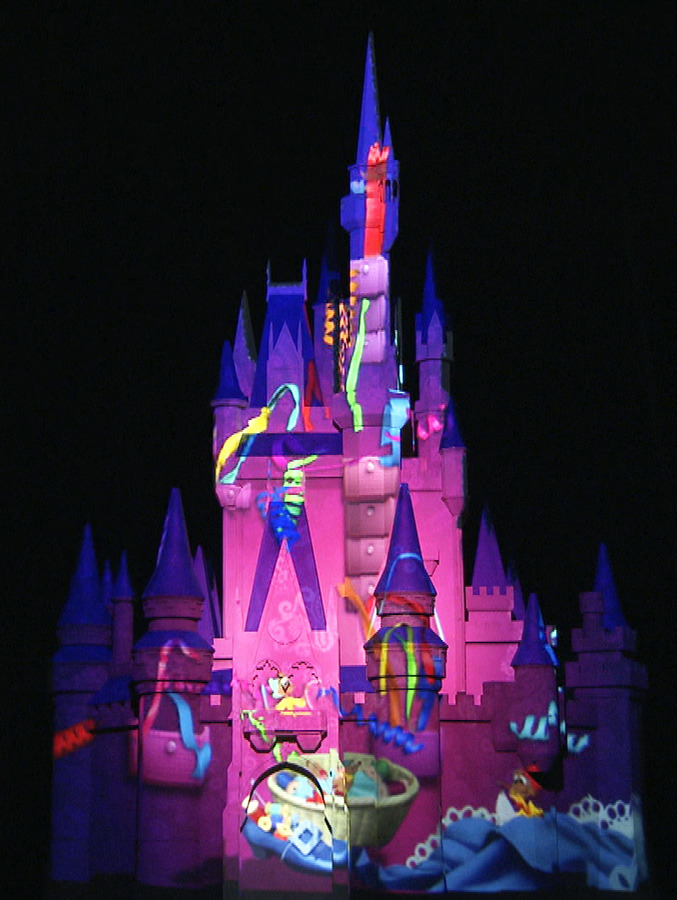
\includegraphics[width=9cm]{image/disney.jpg}
  \caption[東京ディズニーランド Once upon a time]{東京ディズニーランド Once upon a time\cite{disney}.}
\label{disney}
\end{figure}

\begin{figure}[b]
    \centering
    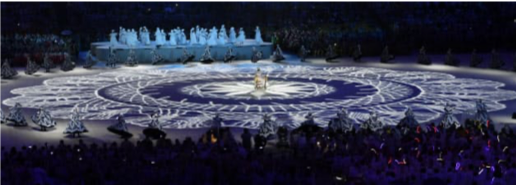
\includegraphics[width=9cm]{image/rio.png}
    \caption[リオオリンピック]{リオオリンピック\cite{rioprojection}.}
  \label{rio}
\end{figure}

\clearpage

\begin{figure}[t]
    \centering
    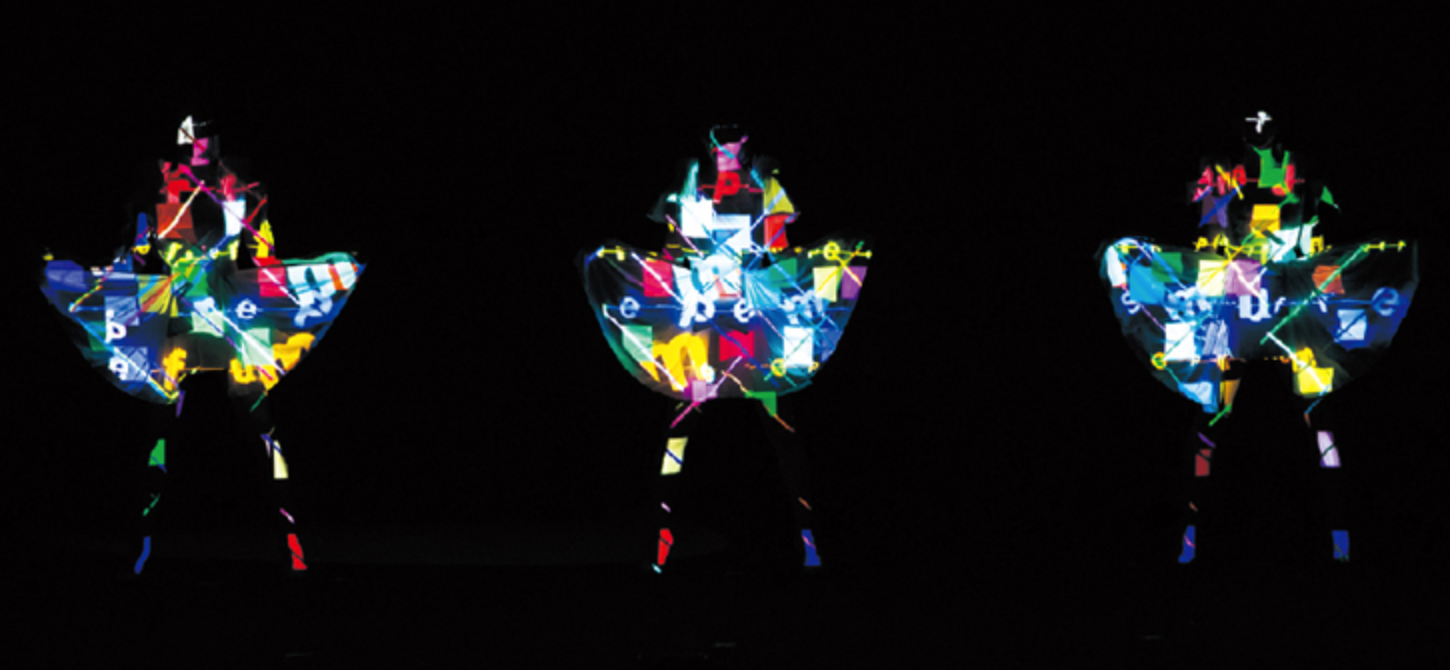
\includegraphics[width=9cm]{image/perfume1.png}
    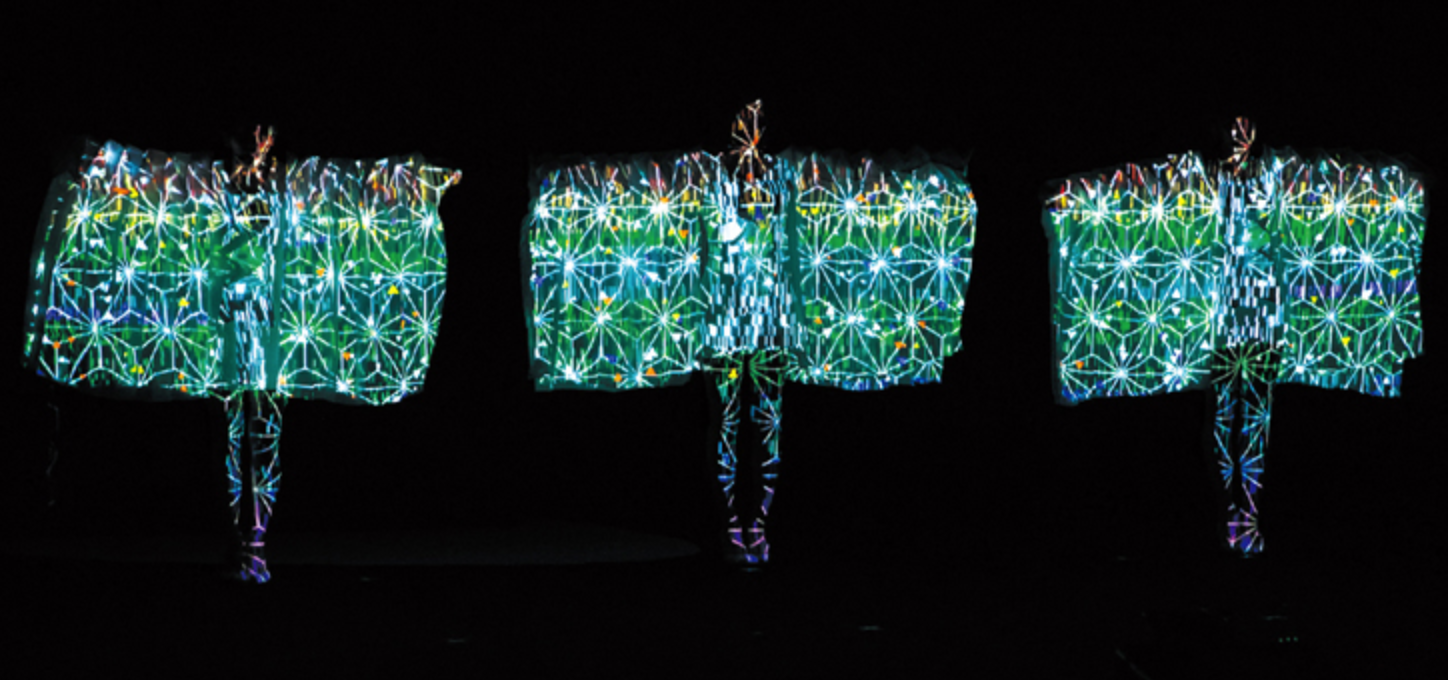
\includegraphics[width=9cm]{image/perfume2.png}
    \caption[Perfume カンヌライオンズ 国際クリエイティビティ・フェスティバル]{Perfume カンヌライオンズ 
    \protect\linebreak 国際クリエイティビティ・フェスティバル\cite{kirameku}.}
  \label{perfume}
\end{figure}



\begin{figure}[b]
  \centering
  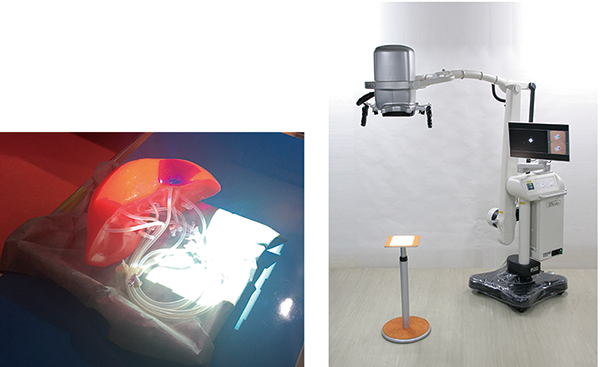
\includegraphics[width=9cm]{image/syujutsu.png}
  \caption[肝臓のICG発光をもとに切離線を決め,修正しながら手術が可能]{肝臓のICG発光をもとに切離線を決め,
  \protect\linebreak 修正しながら手術が可能\cite{iryou}.}
\label{syujutsu}
\end{figure}



%%%%%% 3. 提案手法 %%%%%%
\chapter{提案手法}
\thispagestyle{fancy}

\section{使用装置}
\subsection{Kinect for Windows}
Microsoftから販売された,コントローラーを用いずに身体の動き,ジェスチャー,音声などによって
操作を可能にする周辺機器である.

Kinectには,赤外線センサー,8ビット3チャンネル(RGB)の画像データを取得するRGBカメラ,
Kinectからの距離(深度)の画像データを取得する深度画像センサー,音の発生場所を求める
音源位置推定が可能な音声マイクが搭載されている.
また,Kinectの最も特徴的な機能が「姿勢認識技術」である,人間の全身を認識してその動きによる操作をしている.
これにより,深度画像をもとに,人体のパーツがどこにあるのかを推測することができる\cite{kinect}.

本研究では,Kinect for Windows v1を使用した.

\begin{figure}[b]
    \centering
    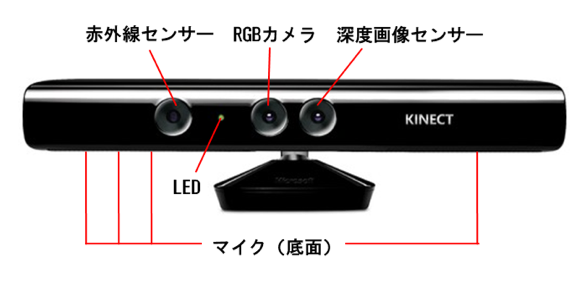
\includegraphics[width=9cm]{image/kinect.png}
    \caption[Kinect for Windows]{Kinect for Windows\cite{kinect}.}
  \label{kinect}
\end{figure}

\clearpage

\subsection{プロジェクター}
投影を行う際に使用した.

\vspace{1cm}
\begin{figure}[h]
    \centering
    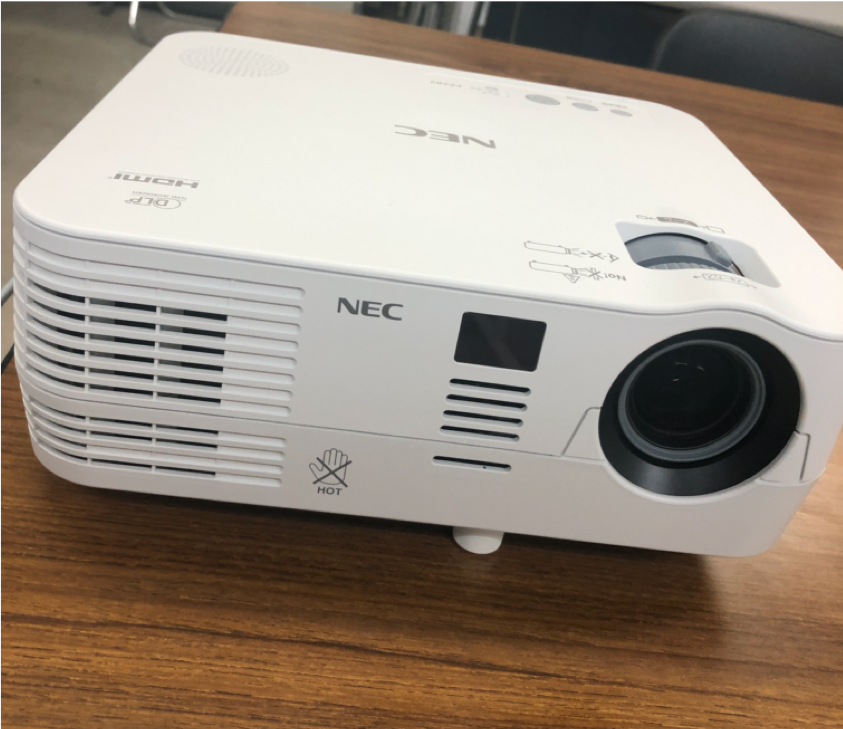
\includegraphics[width=8cm]{image/projector.png}
    \caption[プロジェクター]{プロジェクター.}
  \label{projector}
\end{figure}
\vspace{1cm}


\section{開発環境}
以下の開発環境で実装した.

\begin{itemize}
    \item OS: Windows 10
    \item IDE: Visual Studio 2017
    \item プログラミング言語: C++
    \item ライブラリ: OpenNI2, NiTE2, OpenCV, OpenGL
\end{itemize}

\subsection{OpenNI2}
OpenNI2はPrimeSence社が中心となって開発したオープンソースのライブラリである\cite{motion}.

\subsection{NiTE2}
NiTE2とは,OpenNI2同様,PrimeSence社が提供している姿勢認識ライブラリであり,
OpenNI2のミドルウェアとして利用する.機能として,人の検出,骨格検出,ポーズの検出,
ジェスチャーの検出などがある\cite{motion}.

\subsection{OpenCV}
OpenCV(Intel Open Source Coumputer Vision Library)は,Intelによって開発された無償の
画像処理ライブラリ集であり,画像の変形やテンプレートマッチング,パターン認識,動画解析等の画像処理
アルゴリズムが数多く用意されている.静止画だけでなく動画像やビデオカメラからの入力にも対応しているため,
パソコンのスペックやアルゴリズムによってはリアルタイムで処理することができる\cite{opencv}.

\subsection{OpenGL}
OpenGL\cite{opengl3d}\cite{openglprogram}は,
ワークステーションやパソコンにグラフィックスを表示するための
ソフトウエア・インターフェース(デブス・バッファ法による三次元グラフィクス・ライブラリー)である.
そしてOpenGLは照光処理,シェーディング,テクスチャ・マッピング,陰面除去,
アニメーション機能を備えているインターフェースであり,非常に高品質のグラフィックス表示を
可能とするものである\cite{opengl}.

\clearpage

\section{システムの概要}
本研究では,スポーツに焦点を当て,野球とサッカーの動作を行うことができる
プロジェクションマッピングを実装した.

ユーザに図\ref{combination}のCombination画面の投影を行い,
ユーザのスケルトン座標に応じてインタラクティブに
プロジェクションマッピングを変化させる\cite{busan}\cite{ijrte}.



\subsection{表示画面}
以下の9つの画面を出力する.

\begin{itemize}
    \item Ball画面: スポーツで用いるボール(図\ref{ball})
    \item Color画面: RGBカメラの映像(図\ref{color})
    \item Depth画面: 深度カメラの映像(図\ref{depth})
    \item User画面: 人領域の映像(図\ref{user})
    \item Combination画面: 投影用(図\ref{combination})
    \item Combination\_PC画面: PC用(図\ref{combination})
    \item Skeleton画面: 人の骨格情報(図\ref{skeleton})
    \item Gray画面: Color画面にグレースケールを実行した画面(図\ref{gray})
    \item Cascade画面: 黒い背景画像にGray画面を合成した画面(図\ref{cascade})
\end{itemize}

\clearpage

\begin{figure}[p]
    \begin{minipage}{0.5\hsize}
     \begin{center}
      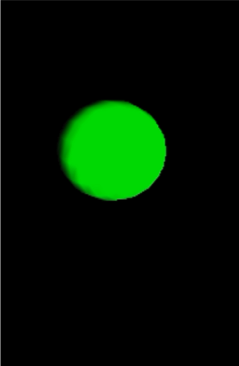
\includegraphics[width=4cm,height=6cm]{image/ball.png}
     \end{center}
     \caption[Ballの画面表示]{Ballの画面表示.}
     \label{ball}
    \end{minipage}
    \begin{minipage}{0.5\hsize}
     \begin{center}
      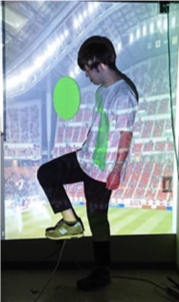
\includegraphics[width=4cm,height=6cm]{image/color.png}
     \end{center}
     \caption[Colorの画面表示]{Colorの画面表示.}
     \label{color}
    \end{minipage}
\end{figure}

\begin{figure}[p]
    \begin{minipage}{0.5\hsize}
     \begin{center}
      \includegraphics[width=4cm,height=6cm]{image/Depth.png}
     \end{center}
     \caption[Depthの画面表示]{Depthの画面表示.}
     \label{depth}
    \end{minipage}
    \begin{minipage}{0.5\hsize}
     \begin{center}
      \includegraphics[width=4cm,height=6cm]{image/User.png}
     \end{center}
     \caption[Userの画面表示]{Userの画面表示.}
     \label{user}
    \end{minipage}
\end{figure}

\clearpage

\begin{figure}[p]
    \begin{minipage}{0.5\hsize}
     \begin{center}
      \includegraphics[width=4cm,height=6cm]{image/Combination.png}
     \end{center}
     \caption[CombinationとCombination\_PCの画面表示]{CombinationとCombination\_PCの画面表示.}
     \label{combination}
    \end{minipage}
    \begin{minipage}{0.5\hsize}
     \begin{center}
      \includegraphics[width=4cm,height=6cm]{image/Skeleton.png}
     \end{center}
     \caption[Skeletonの画面表示]{Skeletonの画面表示.}
     \label{skeleton}
    \end{minipage}
\end{figure}

\begin{figure}[p]
    \begin{minipage}{0.5\hsize}
     \begin{center}
      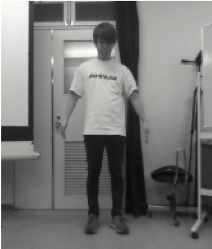
\includegraphics[width=4cm,height=6cm]{image/gray.png}
     \end{center}
     \caption[Grayの画面表示]{Grayの画面表示.}
     \label{gray}
    \end{minipage}
    \begin{minipage}{0.5\hsize}
     \begin{center}
      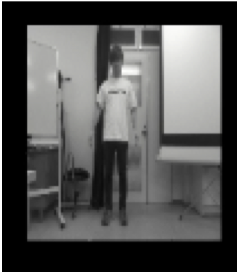
\includegraphics[width=4cm,height=6cm]{image/cascade.png}
     \end{center}
     \caption[Cascadeの画面表示]{Cascadeの画面表示.}
     \label{cascade}
    \end{minipage}
\end{figure}

\clearpage

\subsection{スケルトンナンバー}
Kinect for Windows v1において,スケルトンナンバーは図\ref{num}に示すように割り当てられている.

\begin{figure}[htbp]
    \centering
    \includegraphics[height=7cm]{image/Skeleton_num.png}
    \caption[スケルトンナンバー]{スケルトンナンバー.}
  \label{num}
\end{figure}

\vspace{1cm}

\begin{table}[h]
    \centering
    \begin{tabular}{|lc|lc|} \hline
      0 & 頭 & 8 & 胴体 \\ 
      1 & 首 & 9 & 左腰 \\
      2 & 左肩 & 10 & 右腰 \\
      3 & 右肩 & 11 & 左膝 \\
      4 & 左肘 & 12 & 右膝 \\
      5 & 右肘 & 13 & 左足 \\
      6 & 左手 & 14 & 右足 \\
      7 & 右手 &  &  \\ \hline
    \end{tabular}
    \caption[スケルトンナンバーと体の位置関係]{スケルトンナンバーと体の位置関係.}
    \label{numtable}
\end{table}

\clearpage

システム起動時のスケルトン認識の不安定さを防ぐために,
ユーザは「気を付け」のポーズをとる事とする.
このポーズは以下に示す状態のポーズとする(図\ref{num}参照).


\begin{enumerate}
    \item 左肩と右肩の$y$座標の差が$420mm$未満
    \item 左肘と右肘の$y$座標の差が$450mm$未満
\end{enumerate}

\vspace{1cm}

\begin{figure}[h]
    \centering
    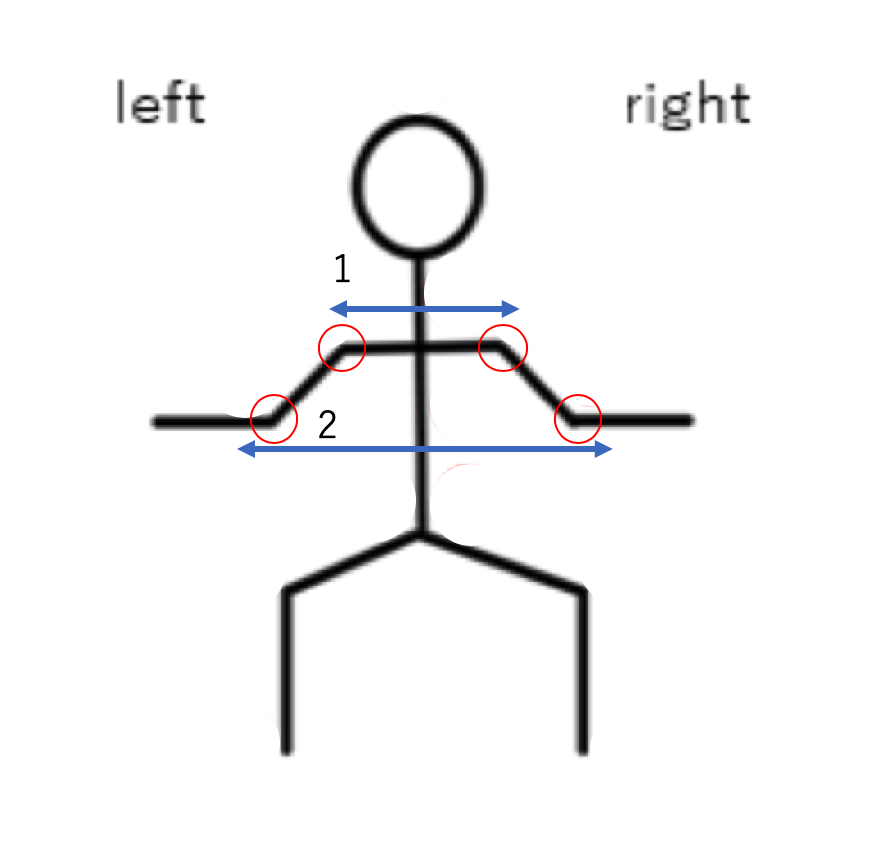
\includegraphics[width=8cm]{image/kiwotsuke.png}
    \caption[「気を付け」のポーズ]{「気を付け」のポーズ.}
  \label{kiwotsuke}
\end{figure}
\vspace{1cm}

それぞれのモードにおいて,一連の動作が終了すると初期化を行う.
それによって,連続して投影を行うことを可能にした.

それぞれのモードに切り替わる前は,画面は黒い初期画面である.

\clearpage

\subsection{野球モード}
ピッチングの一連の動作を行う際に,野球ボールと野球場の投影を行う.

\vspace{1cm}
\begin{figure}[h]
    \centering
    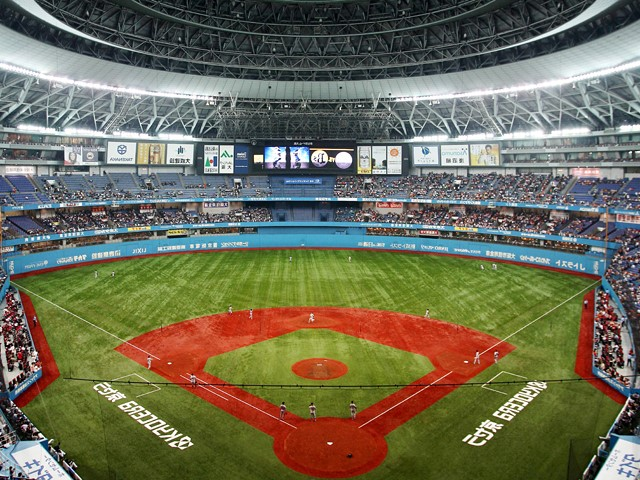
\includegraphics[width=9cm]{image/baseball_back.jpg}
    \caption[野球モードの背景画像]{野球モードの背景画像\cite{baseballback}.}
  \label{baseballback}
\end{figure}
\vspace{1cm}

ボールは投げる際に音がなり,飛距離が伸びるにつれ,徐々に小さくする事で実際にボールを投げたかのような演出を行う.
ボールの位置が$x$座標のしきい値(被験者から見て画面左端)より大きくなった場合,ボールは消えて初期化される.


\clearpage

以下にピッチングの手順を示す.

\begin{enumerate}
    \item 胸の付近で両手を構える(以下の6つの条件を満たす必要がある)
        \begin{itemize}
            \item 左肘の$x$座標と胴の中心の$x$座標の差が$200mm$未満
            \item 左肘の$y$座標と胴の中心の$y$座標の差が$200mm$未満
            \item 右肘の$x$座標と胴の中心の$x$座標の差が$200mm$未満
            \item 右肘の$y$座標と胴の中心の$y$座標の差が$200mm$未満
            \item 首の$y$座標と左手の$y$座標の差が$200mm$未満
            \item 首の$y$座標と右手の$y$座標の差が$200mm$未満
        \end{itemize}
    \item 頭より上に来るように右(左)手を振り上げるとボールが出現し動き出す(以下の条件で認識する).
        \begin{itemize}
            \item 振り上げた右(左)手の$y$座標が頭の中心の$y$座標よりも高い
        \end{itemize}
\end{enumerate}


\vspace{1cm}
\begin{figure}[h]
    \centering
    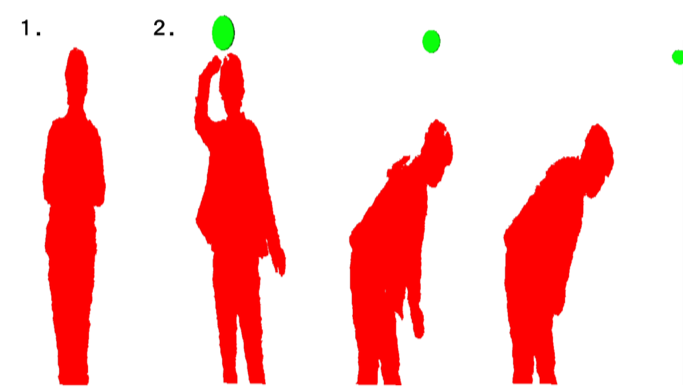
\includegraphics[width=8cm]{image/baseball.png}
    \caption[野球モードを実行した際のCombinationの画面表示]{野球モードを実行した際のCombinationの画面表示.}
  \label{baseball}
\end{figure}
\vspace{1cm}

\clearpage

\subsection{サッカーモード}
リフティングの一連の動作を行う際に,サッカーボールとサッカー場の投影を行う.
\vspace{1cm}
\begin{figure}[h]
    \centering
    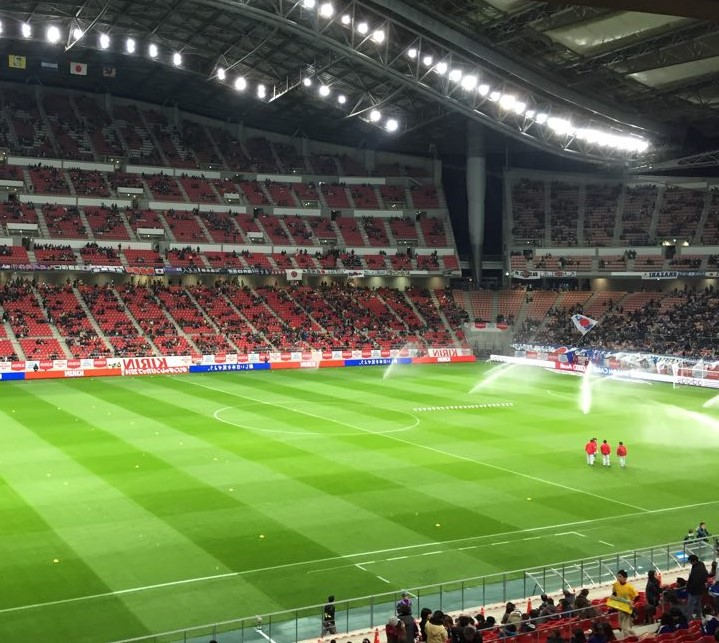
\includegraphics[width=9cm]{image/soccer_back.jpg}
    \caption[サッカーモードの背景画像]{サッカーモードの背景画像.}
  \label{soccerback}
\end{figure}
\vspace{1cm}

ボールは蹴り上げる際には音がなる.また,
ボールの位置が$y$座標のしきい値(画面下)より低くなった場合,ボールは消え初期化される.


\clearpage
以下にリフティングの手順を示す.

\begin{enumerate}
    \item 右(左)膝を右(左)腰ほどの高さになるように蹴り上げるとボールが出現する(以下の条件で認識する).
        \begin{itemize}
            \item 右(左)膝の$y$座標が右(左)腰から$300mm$低い位置より高く蹴り上げると,ボールが出現し動き出す.            
        \end{itemize}
    \item 右(左)膝を下ろすとボールは下がり続ける.
\end{enumerate}

\vspace{1cm}
\begin{figure}[h]
    \centering
    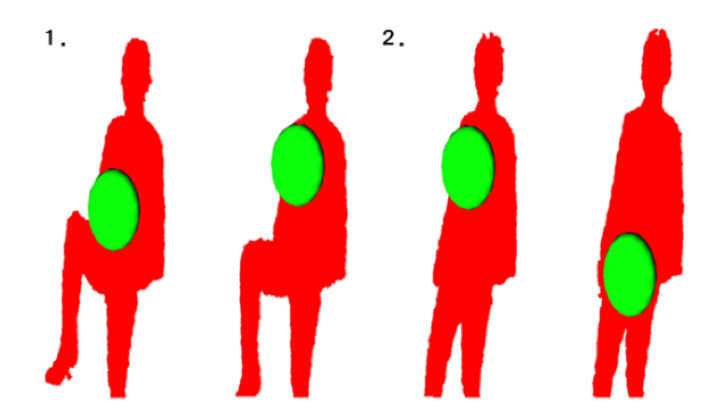
\includegraphics[width=8cm]{image/soccer.png}
    \caption[サッカーモードを実行した際のCombinationの画面表示]{サッカーモードを実行した際のCombinationの画面表示.}
  \label{baseball}
\end{figure}

\vspace{1cm}

また,リフティングの動きは,次の物理演算を使用している.

$y$座標は上向きを正とし,プロジェクションマッピングの画面中央を$y=0$とする.

\clearpage

\begin{figure}[h]
    \centering
    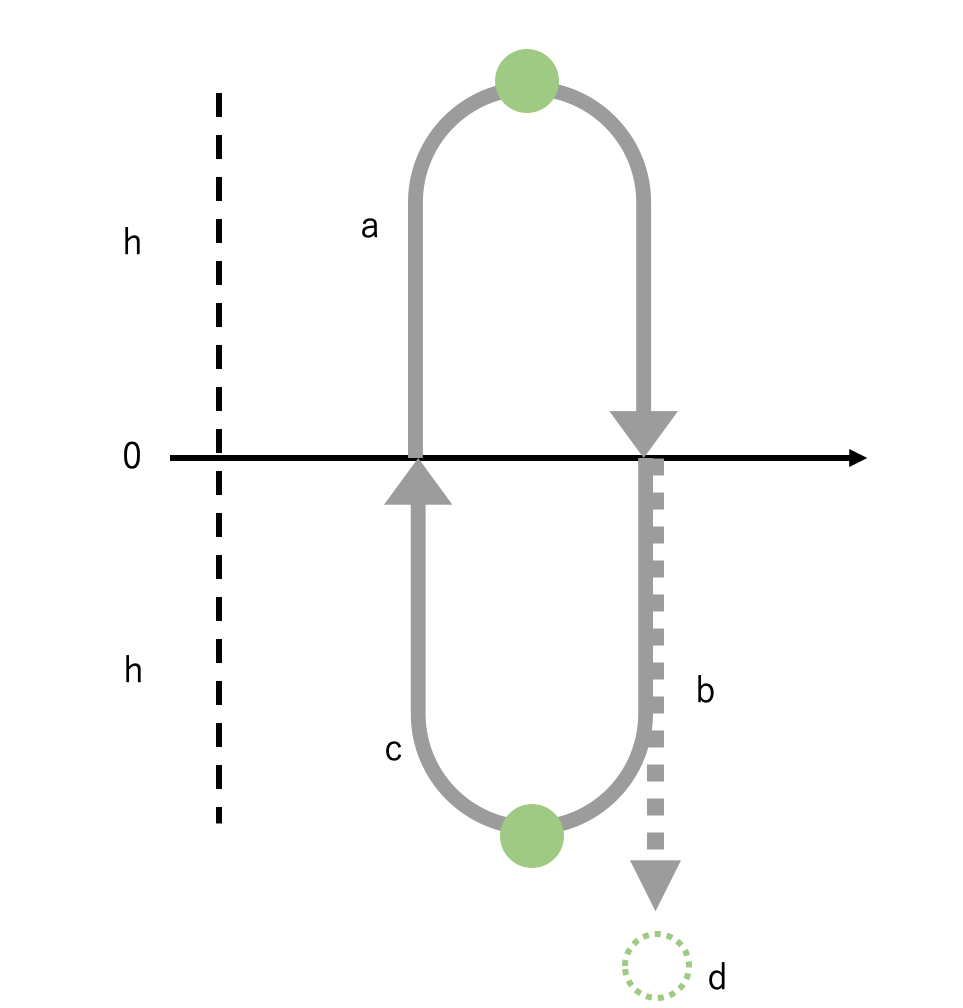
\includegraphics[width=9cm]{image/butsuri2.png}
    \caption[リフティングのボールの動き]{リフティングのボールの動き.}
  \label{butsuri}
\end{figure}



\[
    \begin{cases}
        v_0,v_0': 初速度 & \\
        t: 時間 & \\
        g: 重力加速度(g=9.8)とする. &
    \end{cases}
\]

\vspace{1cm}

\begin{itemize}
    \item[a] ボールの位置が$y \geqq 0$の場合
        \begin{equation}
            y=v_0t-\frac{1}{2}gt^2
        \end{equation}
        \begin{equation}
            v_0=25とすると,y=25t-\frac{1}{2}gt^2
        \end{equation}
    \item[b,c] ボールの位置が$y < 0$の場合
        \begin{itemize}
            \item[b] 一定速度で落下
            \item[c] ボールを蹴り上げる動作をした時
                \begin{equation}
                    y=v_0't-\frac{1}{2}gt^2
                \end{equation}
        \end{itemize}
\end{itemize}

\vspace{1.5cm}

\begin{figure}[htbp]
    \centering
    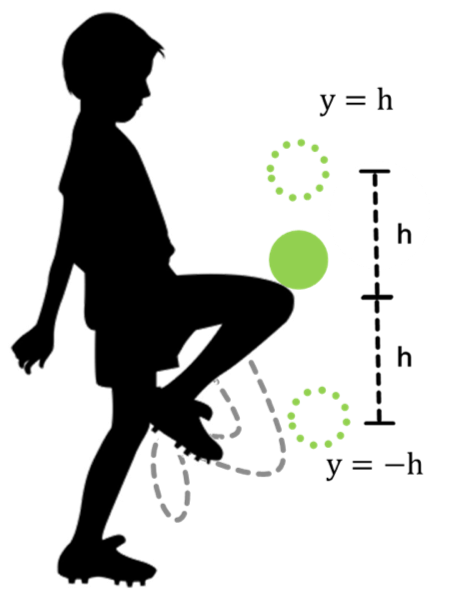
\includegraphics[width=6cm]{image/ballenzan.png}
    \caption[ボールを蹴り上げた時点でのボールの位置]{ボールを蹴り上げた時点でのボールの位置.}
  \label{enzan}
\end{figure}

\vspace{1cm}


\begin{itemize}
    \item ボールの最高点の位置をy=h(図\ref{butsuri}参照)
    \item ボールを蹴り上げた時点でのボールの位置をy=-h(図\ref{butsuri},図\ref{enzan}参照)と仮定
\end{itemize}


連続したリフティング動作を行えるようにするため,aでのボールの最高点に,
再び蹴り上げたボールの高さをそろえる.これを実現させるため,以下の計算を行う(図\ref{butsuri}参照).


\begin{itemize}
    \item[aより]
        \begin{equation}
            v^2-v_0^2=2(-g)h
        \end{equation}

        最高点の速さは$v=0$より 

        \begin{equation}
            0-v_0^2=2(-g)h
        \end{equation}

        よって

        \begin{equation}
            v_0=\sqrt{2gh}
        \end{equation}

    \item[cより]
        \begin{equation}
            v^2-v_0'^2=2(-g)(2h)
        \end{equation}

        最高点の速さは$v=0$より 

        \begin{equation}
            0-v_0'^2=2(-g)(2h)
        \end{equation}
        よって

        \begin{equation}
            v_0'=\sqrt{4gh}
        \end{equation}

    \item[以上より]
        \begin{equation}
            v_0'=\sqrt{2}v_0
        \end{equation}

        よって$v_0'$は$v_0$の$\sqrt{2}$倍である. 

        \begin{equation}
            v_0'=25*\sqrt{2} \fallingdotseq 35.4 
        \end{equation}

        より

        \begin{equation}
            y=35.4*t-\frac{1}{2}gt^2
        \end{equation}

    \item[dより] ボールが閾値(画面下)より低くなった場合ボールは消える. 

\end{itemize}

\vspace{1.5cm}


\clearpage

\subsection{カスケード分類器を用いたユーザのポーズ認識}
Kinectには,スケルトントラッキングの対象となる人物を認識した
人物から無作為に選択する問題が存在している\cite{hitogomi}.
骨格座標を用いた手法では,ユーザがKinectの視野から隠れた後,再度Kinectの視野内に
入った場合,ユーザの骨格座標の再追従が上手く行われない問題があった\cite{beppu}.
その問題を解決する手段として,図\ref{cascade}のCascade画面に
カスケード分類器を用いてユーザの検出を行う手法を提案する.




\subsubsection{AdaBoost}
ブースティングは,弱い分類器を順次生成し,
それらを組み合わせて強い分類器を作成する学習アルゴリズムである\cite{boosting}.

本研究では,さまざまなブースティング手法の中でAdaBoostと呼ばれる手法を使用した.
AdaBoostは,学習プロセス中に分類器の認識率に適応的に重み付けすることにより学習することにより,
高精度で分類器を作成する手法である\cite{adaboost}.

図\ref{adaboost}において,$h_T(x)$は$T$個目の特徴量を指し,$\alpha$は重みを指す.

\vspace{1.2cm}


\begin{figure}[h]
    \centering
    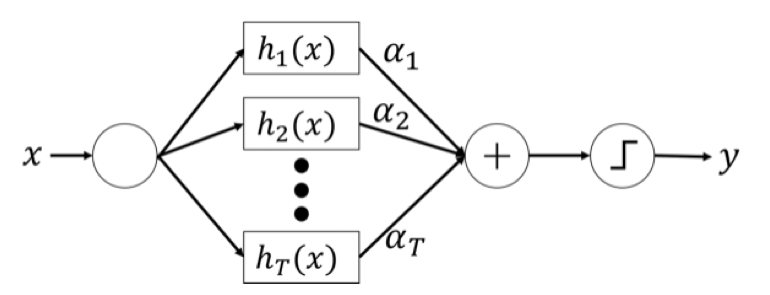
\includegraphics[width=12cm]{image/adaboost.png}
    \caption[AdaBoost]{AdaBoost\cite{adafig}.}
  \label{adaboost}
\end{figure}

\vspace{1.2cm}

\clearpage
\begin{itemize}
    \item ブースティングのおおまかな流れ\cite{suugaku}
        \begin{enumerate}
            \item $弱学習器h_1(x)を作る$
            \item $h_1(x)の結果を考慮して,次の弱学習器h_2(x)を作る$
            \item $以下順々に,h_{t-1}(x)の結果を考慮して,次の弱学習器h_tを作る$
            \item $h_Tまで作ったらh_1(x)からh_T(x)までをまとめて強学習器h(x)を作る$
        \end{enumerate}
    
    \item AdaBoostの重み
        \begin{itemize}
            \item 各学習器の重み$\alpha_t$の決め方($E_t$: 学習器$h_t$の誤差)
                \begin{equation}
                    \alpha_t=\frac{1}{2}\ln(\frac{1-E_t}{E_t})
                \end{equation}
                

                $h_t$の誤分類が大きくなればなるほど,$\alpha_t$が小さくなり$h_t$の重要度は小さくなる.

            \item $t$回目の学習におけるサンプル$i$の重み$w_i^{(t)}$の決め方
                \begin{equation}
                    w_i^{(t)}=C_tw_i^{(t-1)}e^{-y_i\alpha_th_t(x_i)}
                \end{equation}
            
        \end{itemize}
\end{itemize}


\subsubsection{画像の特徴抽出}
カスケード分類器は,学習時に特徴量の抽出を行う. 
以下に3つの特徴量の抽出方法を示す.

\begin{itemize}
    \item Haar-like特徴量
    \item Local Binary Pattern (LBP)特徴量
    \item Histogram of Oriented Gradients (HOG)特徴量
\end{itemize}

本研究では,LBP特徴量を用いた.


\clearpage
\subsubsection{LBP特徴量}
LBPとは,画像の認識と分類に使用できる特徴量の1つである\cite{adafig}\cite{lbp}.
LBPは回転変動などには弱いが,照明変化の影響を受けにくく,また高速計算が可能といった特徴がある.

LBPの計算は$3*3$ピクセルサイズの画素領域に着目し行う.
まず中心の輝度値と周辺8近傍の画素の輝度値を比較する.その8近傍の内,
輝度値が中心の輝度値以上のとき1,それ以外を0とする.ここにマスクを掛け合わせ,
その総和を求めこの値が中心画素の輝度値と置き換える. 
マスクとは,左上から時計回りに$2^n$の重みを割り振ったものである (図\ref{lbpfig}中,右から2番目の図).
この作業を全画素に対して行い,できた画像をLBP画像と呼ぶ.
こうして求めたLBP特徴量を用いて物体を認識する.

\vspace{1.5cm}

\begin{figure}[h]
    \centering
    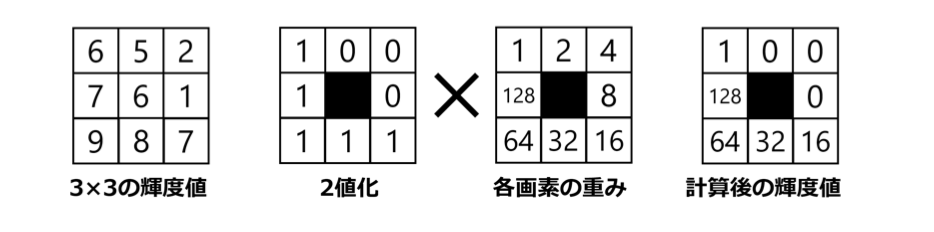
\includegraphics[width=13cm]{image/lbpfig.png}
    \caption[LBPの計算方法]{LBPの計算方法\cite{adafig}.}
  \label{lbpfig}
\end{figure}

%\begin{equation}
%    LBP=1+16+32+64+128=241
%\end{equation}

\clearpage
\subsubsection{サッカーモードにおけるカスケード分類器の作成}
サッカーモードにおいて,ユーザが膝でボールを蹴り上げている動作を行っている
画像をポジテイブ画像,
ユーザがそれ以外の動作を行っている画像をネガテイブ画像として学習を行いカスケード分類器を作成した.

\vspace{1.5cm}

\begin{figure}[h]
    \begin{minipage}{0.5\hsize}
     \begin{center}
      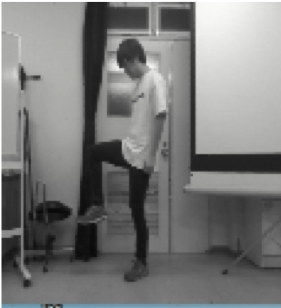
\includegraphics[width=3cm,height=4cm]{image/posi.png}
     \end{center}
     \caption[ポジティブ画像]{ポジティブ画像.}
     \label{posi}
    \end{minipage}
    \begin{minipage}{0.5\hsize}
     \begin{center}
      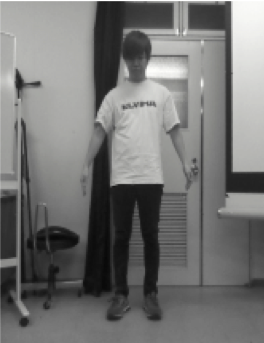
\includegraphics[width=3cm,height=4cm]{image/nega2.png}
     \end{center}
     \caption[ネガティブ画像]{ネガティブ画像.}
     \label{nega}
    \end{minipage}
\end{figure}

\vspace{1cm}

\begin{table}[htb]
    \centering
     \begin{tabular}{cc}	\hline
       ポジティブ画像 & ネガティブ画像 \\	\hline \hline
       1200 & 345 \\\hline
     \end{tabular}
    \caption[学習に用いた画像枚数]{学習に用いた画像枚数.}
  \end{table}


\clearpage
カスケード分類器を用いたサッカーモードのユーザ認識の図を以下に示す.

\vspace{1cm}


\begin{figure}[h]
  \centering
  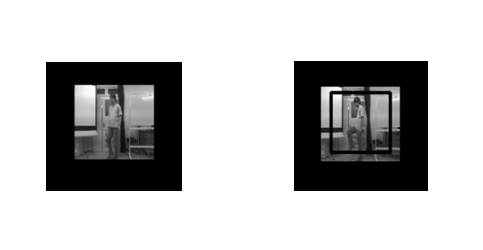
\includegraphics[width=9cm]{image/ninshiki.png}
  \caption[カスケード分類器を用いたサッカーモードのユーザ認識]{カスケード分類器を用いたサッカーモードのユーザ認識.}
\label{lbpfig}
\end{figure}





%%%%%% 4. 実行結果 %%%%%%
\chapter{実行結果}
\thispagestyle{fancy}

\section{実行結果}
以下にサッカーモードと野球モードの実行結果を示す.
\begin{itemize}    
    \item サッカーモード
        \begin{figure}[htbp]
            \centering
            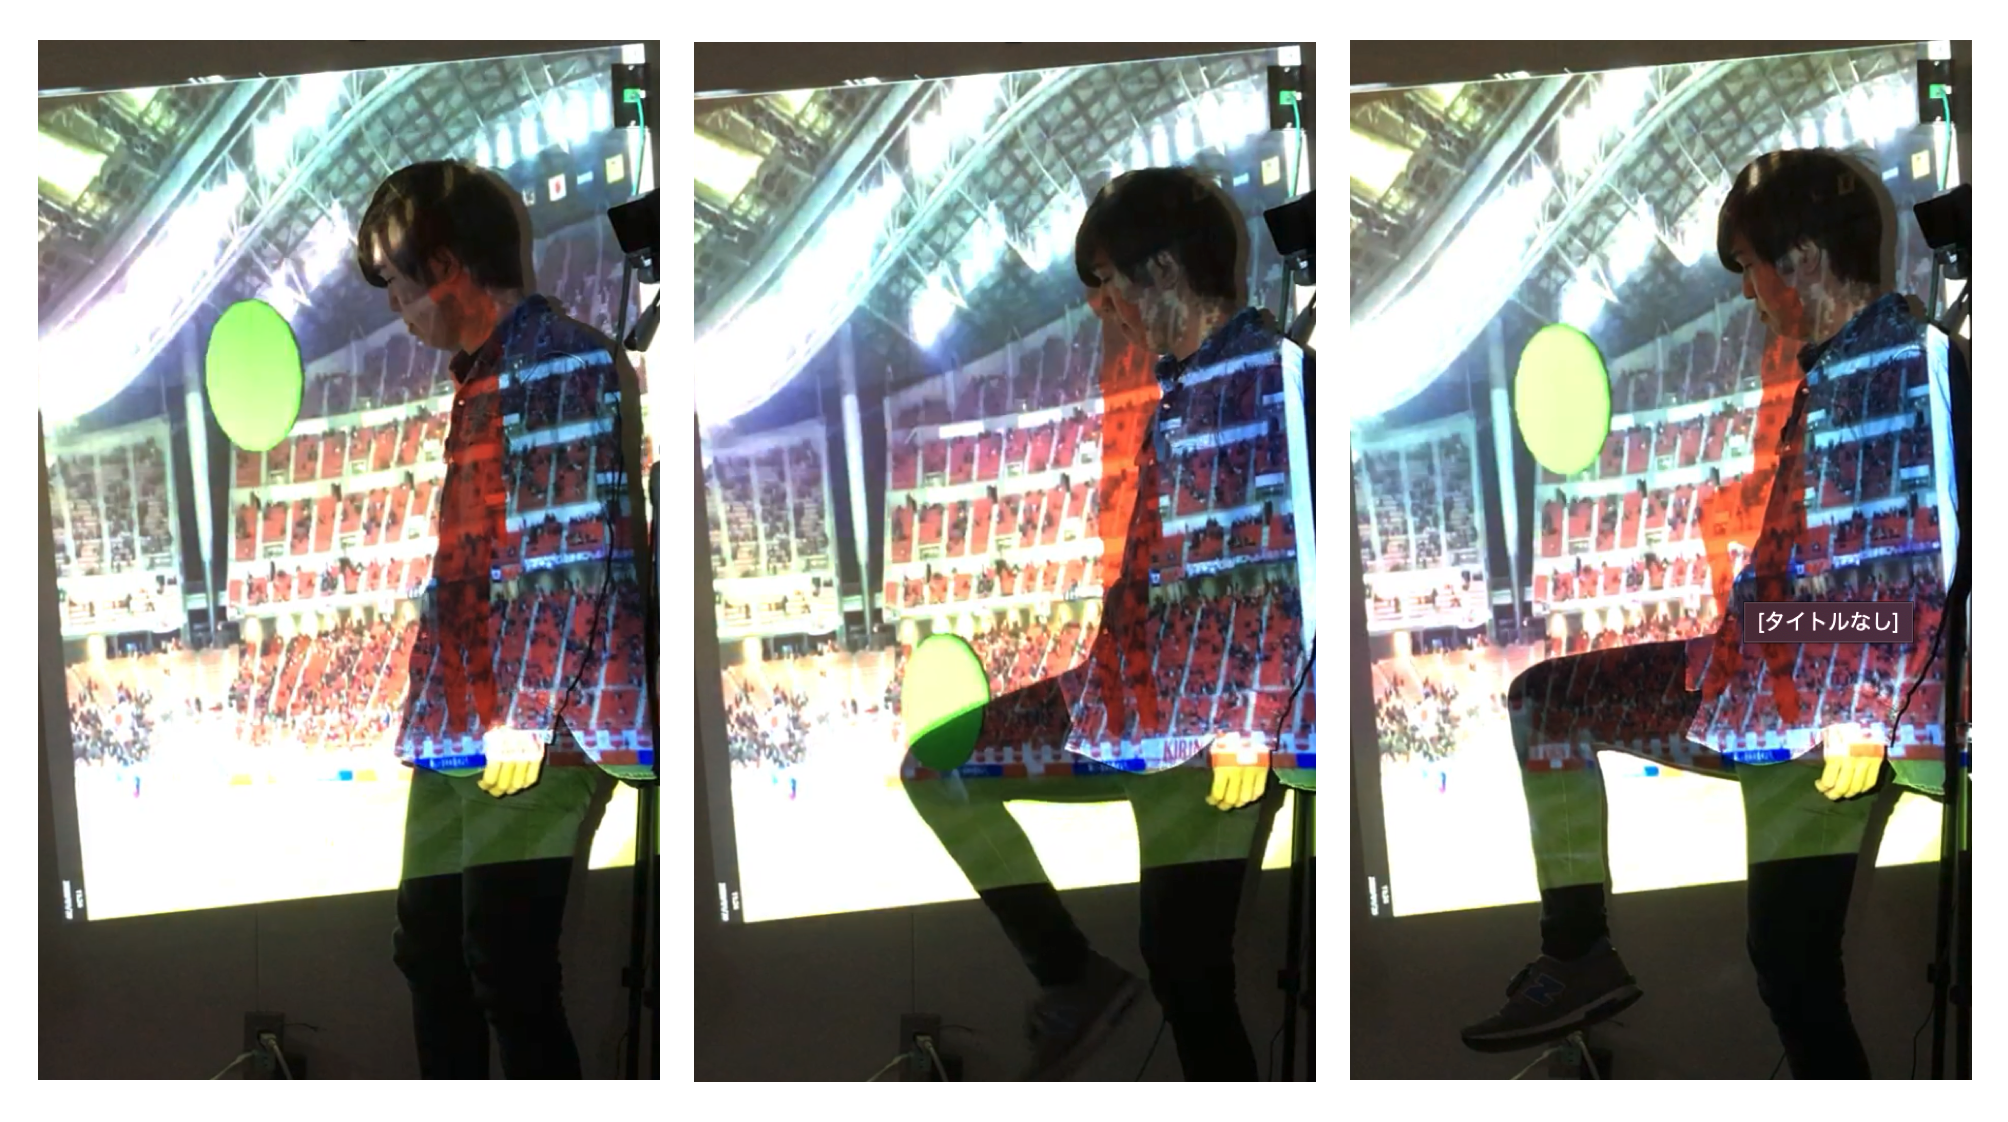
\includegraphics[width=12cm]{image/soccer_kekka.png}
            \caption[サッカーモードの実行結果]{サッカーモードの実行結果.}
            \label{soccer_kekkka}
        \end{figure}

\clearpage

    \item 野球モード
        \begin{figure}[htbp]
            \centering
            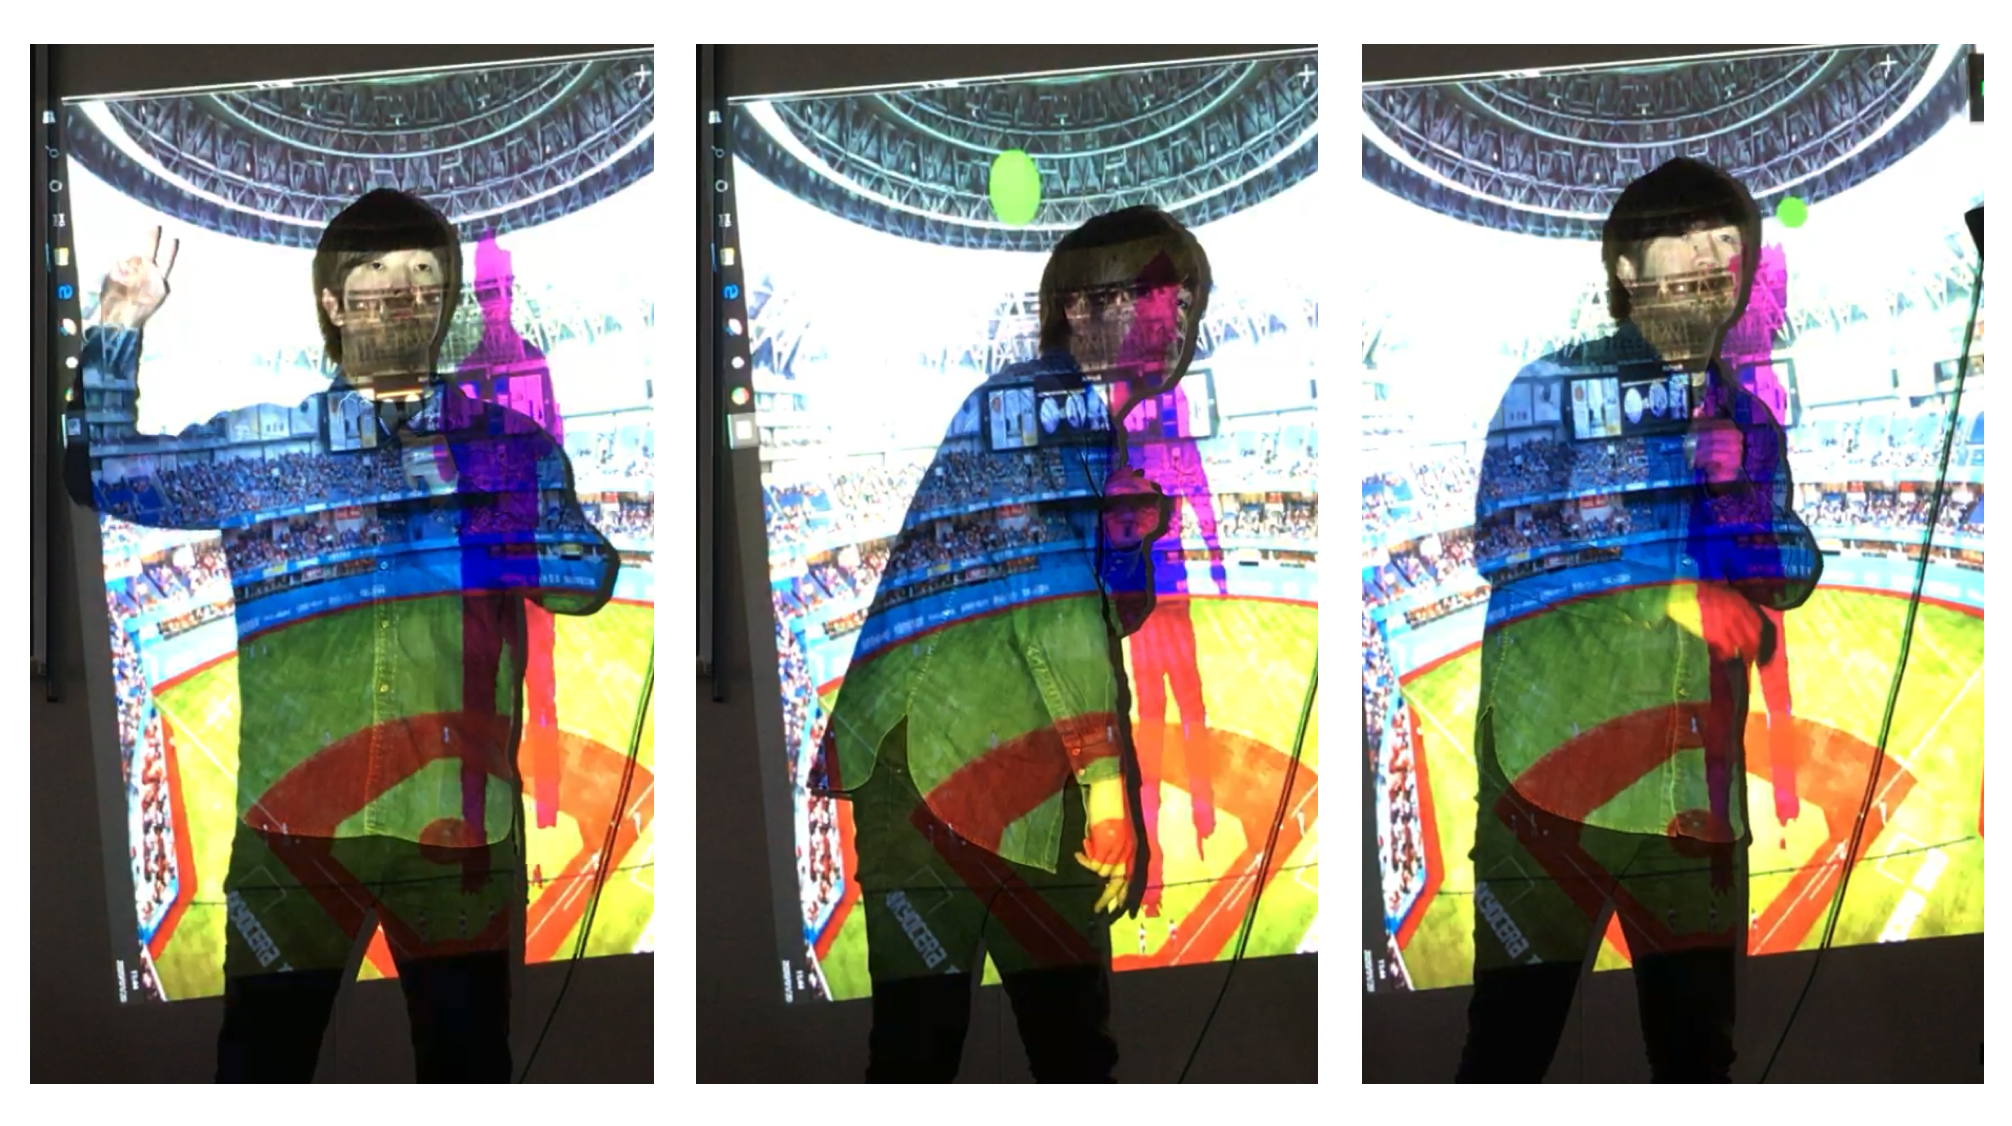
\includegraphics[width=12cm]{image/baseball_kekka.png}
            \caption[野球モードの実行結果]{野球モードの実行結果.}
        \label{baseball_kekka}
        \end{figure}
\end{itemize}

%%%%%% 5. 評価 %%%%%%
\chapter{評価実験}
\thispagestyle{fancy}


\section{評価実験}
サッカーモードにおけるカスケード分類器ごとの認識率などの評価にする?

ユーザによるアンケート評価?

背景に考慮するためにuser画面を用いた実験を行ったがうまくいかなかった.


サッカーモードに使用する学習データを以下に示す.

\begin{table}[h]
    \centering
    \scalebox{1.0}[1.0]{
     \begin{tabular}{cc}	\hline
       ポジティブ画像 & 771  \\    
       ネガティブ画像 & 690  \\
       ステージ数 & 13773  \\ \hline
     \end{tabular}
    } 
    \caption{サッカーモードにおける学習データ}
    \label{soccerstudy}
\end{table}


%%%%%% 6. 考察 %%%%%%
\chapter{考察}
\thispagestyle{fancy}

\section{考察}
評価結果より,
プロジェクションマッピングを見る人々だけでなく,
ユーザも楽しめるかについては一定の評価を得る事ができた.

しかし,カスケード分類器を用いた手法では,誤認識があり改善の余地があると考える.





今後の課題としては,アンケートの回答から得られた
チュートリアル画面の実装,
ボールへのテクスチャマッピング,
サッカーモードにおいてリフティング可能部位の増やす,
FPSの向上や,
体の小さな子供や体の不自由な方にも体験してもらえるようにすることなどが挙げられる.

%%%%%% 7. おわりに %%%%%%
\chapter{おわりに}
\thispagestyle{fancy}

\section{おわりに}

本研究では,KinectとOpenCVを用いて,参加型のプロジェクションマッピングを制作した.

%%%%%% 謝辞 %%%%%%
\newpage
\phantomsection
\addcontentsline{toc}{chapter}{謝辞}
\chapter*{謝辞}
\thispagestyle{fancy}
本研究にあたり,丁寧なご指導をして頂いた坂本眞人准教授に
この場を借りて心より御礼申し上げます.
また,様々な意見をくださいました坂本研究室の皆様,
アンケートに協力していただいた情報システム科及び他学科の皆様にも感謝申し上げます.

%%%%%% 参考文献 %%%%%%
\begin{thebibliography}{99}
\thispagestyle{fancy}
%%% 概要 %%%
%\bibitem{hoge} hoge

%%% はじめに %%%
\bibitem{tppm} 小笠航, 片寄晴弘. ``TPPM(Take Part in Projection Mapping):タブレット端末を用いた多人数参加型 プロジェクションマッピングアプリケーション'', 2014年

%%% 先行事例 %%%
\bibitem{once} ``ディズニーランド「ワンス」11月で終了へ'' シネマトゥデイ. [Online] https://www.cinematoday.jp/news/N0090846.
\bibitem{olympic} ``オリンピック大会を支えた製品・技術'', パナソニック. [Online]  https://www.panasonic.com/global/olympic/ja/rio/solution/dlp.html.
\bibitem{amuro} ``自己最長ツアー「LIVE STYLE 2016-2017」に見た、安室奈美恵というパフォーマーの矜持'', SPICE. [Online] https://spice.eplus.jp/articles/116764.
\bibitem{disney} ``[ディズニー]初プロジェクションマッピングに『アリス』『シンデレラ』...知っておきたい6つのポイント3枚目の写真・画像'' cinemacafe.net. [Online] https://www.cinemacafe.net/article/img/2014/05/19/23508/106689.html.
\bibitem{rioprojection} ``リオの会場に咲いたパナのプロジェクションマッピング'' オリパラスポーツイノベーション. [Online] https://style.nikkei.com/article/DGXMZO06971870X00C16A9UP2000/.
\bibitem{kirameku} ``きらめく日本技術'', niponica. [Online] http://web-japan.org/niponica/niponica14/ja/feature/feature03.html.
\bibitem{iryou} ``プロジェクションマッピング技術を手術ナビゲーションシステムに応用'', 国立研究開発法人 日本医療研究開発気候. [Online] https://www.amed.go.jp/pr/2017\_seikasyu\_02-16.html.


%%% 提案手法 %%%
\bibitem{kinect} 西林孝, 小野憲史, ``キネクトハッカーズマニュアル''. ラトルズ. 2011年.
\bibitem{motion} 小川新太, ``モーション・キャプチャ・デバイスを利用した人物追尾ロボット'', 中京大学 情報理工学部 機械情報工学科 2014年度 卒業論文.
\bibitem{opencv} 永田雅人, ``動画像処理ライブラリーOpenCV'', 映像情報メディア学会誌. 2007.
\bibitem{opengl3d} 三浦憲二郎, ``OpenGL 3Dグラフィックス入門'', 朝倉書店. 1995.
\bibitem{openglprogram} クレイトン・ウオルカム, ``Win32 OpenGLプログラミング'', プレンティスホール出版 (1996).
\bibitem{opengl} 中田吉郎, 滝沢俊治, 上林正己, 中野達也, ``OpenGLを用いた生体分子の立体構造表示プログラム'', J. Chem. Software, Vol. 6, No. 4, p. 157–164 (2000).
\bibitem{busan} Makoto Sakamoto, Takahiro Shinoda, Takahiro Ishizu, Masamichi Hori, Amane Takei and  Takao Ito, ``A Proposal of Interactive Projection Mapping Using Kinect'', 2018 International Conference on Information and Communication Technology Robotics (ICT-ROBOT2018), IEEE, Busan, South Korea, DOI: 10.1109/ICT-ROBOT.2018.8549899, September 2018.
\bibitem{ijrte} Makoto Sakamoto, Takahiro Shinoda, Takahiro Ishizu, Amane Takei and Takao Ito, ``Projection Mapping: Interactive Operation using Kinect'', International Journal of Reccent Technology and Engineering (IJRTE) ISSN: 2277-3878, Volume 8, Issue 4, pp.9307-9313, November 2019. 
\bibitem{baseballback} ``Sports Graphic''. NumberWeb. [Online] https://number.bunshun.jp/articles/-/158512.
\bibitem{hitogomi} 濱砂雅人, 伊藤暢浩, 幸塚義之, ``人ごみにおけるKinectセンサの誤認追跡の改善について'', 30th Fuzzy System Symposium, Kochi, September 1-3, 2014.
\bibitem{beppu} Takahiro Shinoda, Makoto Sakamoto, Takahiro Ishizu,  Kenji Sakoma, Amane Takei and Takao Ito, ``Proposal of Interactive Projection Mapping using Human Detection by Machine Learning'', The 2020 International Conference on Artificial Life and Robotics(ICAROB2020), B-Con Plaza, Jan. 13-16, Beppu, Oita, Japan, 2020.
\bibitem{boosting} Nobuyuki Nishiuchi, Takuma Suzuki, Kimihiro Yamanaka ``Development of Work Posture Evaluation System Using Boosting'' J Jpn Ind Manage Assoc 62,51-58,2011.
\bibitem{adaboost} Yoav Freund, Robert E Schapire, ``A Decision-Theoretic Generalization of On-Line Learningand an Application to Boosting'', journal of computer and system sciences 55, 119139 (1997).
\bibitem{suugaku} ``ブースティングとアダブースト(AdaBoost)について詳しく解説'', 具体例で学ぶ数学. [Online] https://mathwords.net/adaboost. 
\bibitem{adafig} 森まどか, 會澤要, 鈴木拓央, 小林邦和 ``カスケード型分類器を用いた照明環境変化にロバストなサッカーボール認識'', 人工知能学会研究会資料. JSAI Technical Report SIG-Challenge-051-5 (5/4).
\bibitem{lbp} Ojala T, Pietikainen M, Harwood D, ``Performance evaluation of texture measures with classification based on Kullback discrimination of distributions.'', Proc. 12th International Conference on Pattern Recognition (ICPR 1994), Jerusalem, Israel. Vol I, 582-585. (1994).


\end{thebibliography}

%%%%%% 付録A %%%%%%
\appendix
\chapter{プログラム}
\thispagestyle{fancy}

本研究で用いたプログラム

\vspace{0.5cm}

main.cpp
\begin{lstlisting}
#pragma comment(linker, "/SUBSYSTEM:WINDOWS /ENTRY:mainCRTStartup")

#include "stdafx.h"

#include<stdio.h>

// OpenNI2 Header file
#include <OpenNI.h> 

// NITE2 Header file
#include <NiTE.h> 

#include <opencv2/opencv.hpp>
#include <opencv/highgui.h>

#include <GL/gl.h>
#include <GL/glu.h>
#include <GL/glut.h>

#include <string.h>

#include <mmsystem.h>

// "winmm.libというライブラリをリンかでリンクする
#pragma comment(lib,"winmm.lib") 

#define RANGE 200


// 画面のサイズ
#define WIDTH 640 
#define HEIGHT 480

// 物理演算
#define g 9.8
#define v0 


#if 1

using namespace cv;
using namespace std;

// ballの平行移動用
float x = 0.0f;
// ボールのx軸の動き
float trans_x = 0.0f; 
// ボールのy軸の動き
float trans_y = 0.0f; 

// ボールの大きさ
float scale_x = 0.2; 
float scale_y = 0.2;
float scale_z = 0.2;

bool flag = false;


// ボール
// ballcolor 緑
GLfloat green[] = { 0.0, 1.0, 0.0, 1.0 }; 
// ライトの位置
GLfloat lightpos[] = { 200.0, 150.0, -500.0, 1.0 }; 

// ボールを出さない
bool baseballFlag = false; 
bool soccerFlag = false;
bool soccerFlag_up = false;
// restart
bool baseballFlag_re = false; 
bool soccerFlag_re = false;


// 物理演算
// 力と加速度
double F, a;
// y座標
double y = 0;
// 時間
double t = 0;


// 背景画像
cv::Mat img, img2;




void printString(float x, float y, char* str, int length) {
	float z = -1.0f;
	glRasterPos3f(x, y, z);

	for (int i = 0; i < length; i++) {
		glutBitmapCharacter(GLUT_BITMAP_HELVETICA_18, str[i]);
	}
}

// 文字列描画
static void DrawString(String str, int w, int h, int x0, int y0)
{
	// 画面上にテキスト描画
	glColor3d(0, 250, 0); 
	// 文字列の位置(左上原点のスクリーン座標系, 文字列の左下がこの位置になる)
	glRasterPos2f(x0, y0); 

	int size = (int)str.size(); // str:文字列
	for (int i = 0; i < size; ++i) {
		char ic = str[i];
		glutBitmapCharacter(GLUT_BITMAP_9_BY_15, ic);
	}
}

// OpenNI2とNITE2を使ってKinectのColor,Depth,User,Skeleton,Combination,Combination_PC,Ballを表示する
void display(void)
{


	// 背景画像を読み込む
	img = cv::imread("baseball_back.jpg", 1);
	img2 = cv::imread("soccer_back.jpg", 1);

	// エラー処理
	if (img.data == NULL) {
		printf("img read error!\n");
	}

	cv::setUseOptimized(true);

	// Initialize OpenNI2
	openni::OpenNI::initialize();

	// Initialize NITE2 
	nite::NiTE::initialize();



	// Device Open
	openni::Status statusOpenNI = openni::STATUS_OK;
	openni::Device device;
	statusOpenNI = device.open(openni::ANY_DEVICE);
	if (statusOpenNI != openni::STATUS_OK) {
		cerr << "Error : openni::Device::open" << endl;
		return;
	}

	// Color Stream Create and Open
	openni::VideoStream colorStream;
	colorStream.create(device, openni::SENSOR_COLOR);
	statusOpenNI = colorStream.start();
	if (statusOpenNI != openni::STATUS_OK) {
		cerr << "Error : openni::VideoStream::start( COLOR )" << endl;
		return;
	}


	// Depth Stream Create and Open
	openni::VideoStream depthStream;
	depthStream.create(device, openni::SENSOR_DEPTH);
	statusOpenNI = depthStream.start();
	if (statusOpenNI != openni::STATUS_OK) {
		cerr << "Error : openni::VideoStream::start( DEPTH )" << endl;
		return;
	}

	// User Tracker Create and Open
	nite::Status statusNITE = nite::STATUS_OK;
	nite::UserTracker userTracker;
	statusNITE = userTracker.create(&device);
	if (statusNITE != nite::STATUS_OK) {
		cerr << "Error : nite::UserTracker::create" << endl;
		return;
	}

	// Setting enable Synchronize
	device.setDepthColorSyncEnabled(true);

	// Set Registration Mode Depth to Color
	// But Kinect doesn't support this Function!
	device.setImageRegistrationMode(openni::IMAGE_REGISTRATION_DEPTH_TO_COLOR);


	cv::Mat grayMat;
	cv::Mat colorMat;
	cv::Mat depthMat;
	cv::Mat userMat;
	cv::Mat skeletonMat;


	// カスケード分類器読み込み
	CascadeClassifier cascade;
	// ここに読み込むカスケード分類器のパスを記述
	cascade.load("");
	// ユーザのポーズ情報を格納場所
	vector<Rect> faces;



	// Windowのサイズ
	cv::namedWindow("Color", cv::WINDOW_NORMAL);
	cv::namedWindow("Gray", cv::WINDOW_NORMAL);
	cv::namedWindow("Depth", cv::WINDOW_NORMAL);
	cv::namedWindow("User", cv::WINDOW_NORMAL);
	cv::namedWindow("Skeleton", cv::WINDOW_NORMAL);

	// Table of Colors
	cv::Vec3b color[7];
	color[0] = cv::Vec3b(255, 255, 255);
	color[1] = cv::Vec3b(255, 0, 0);
	color[2] = cv::Vec3b(0, 255, 0);
	color[3] = cv::Vec3b(0, 0, 255);
	color[4] = cv::Vec3b(255, 255, 0);
	color[5] = cv::Vec3b(255, 0, 255);
	color[6] = cv::Vec3b(0, 255, 255);

	float tmp_x[15];
	float tmp_y[15];
	float tmp_z[15];

	int baseball_status = -1;
	int soccer_status = -1;

	while (1) {
		// Retrieve Frame from Color Stream (8bit 3channel)
		openni::VideoFrameRef colorFrame;
		// Retrieve a Frame from Stream
		colorStream.readFrame(&colorFrame);
		// cv::cvtColor(入力画像, 出力画像, 色空間を変換する値);
		if (colorFrame.isValid()) {
			// Retrieve a Data from Frame 
			colorMat = cv::Mat(colorStream.getVideoMode().getResolutionY(), colorStream.getVideoMode().getResolutionX(), CV_8UC3, reinterpret_cast<uchar*>(const_cast<void*>(colorFrame.getData()))); 
			// Change the order of the pixel RGB to BGR 
			cv::cvtColor(colorMat, colorMat, CV_RGB2BGR); 
			// Change the order of the pixel RGB to GRAY
			cv::cvtColor(colorMat, grayMat, CV_BGR2GRAY); 

		}


		// Retrieve Frame from Depth Stream (16bit 1channel)
		openni::VideoFrameRef depthFrame;
		// Retrieve a Frame from Stream
		depthStream.readFrame(&depthFrame); 
		if (depthFrame.isValid()) {
			// Retrieve a Data from Frame
			depthMat = cv::Mat(depthStream.getVideoMode().getResolutionY(), depthStream.getVideoMode().getResolutionX(), CV_16UC1, reinterpret_cast<ushort*>(const_cast<void*>(depthFrame.getData()))); 
			depthMat.convertTo(depthMat, CV_8UC1, -255.0f / 10000, 255.0);
			// Convert the pixel 0~10000 to 0~255
		}

		// Retrieve User Frame from UserTracker
		nite::UserTrackerFrameRef userFrame;
		// Retrive a Frame form Tracker
		userTracker.readFrame(&userFrame); 
		const nite::UserId* pUserId = userFrame.getUserMap().getPixels();
		// Retrive UserId from Frame
		int width = userFrame.getUserMap().getWidth();
		int height = userFrame.getUserMap().getHeight();
		// 画像を格納する
		userMat = cv::Mat(height, width, CV_8UC3, cv::Scalar(255, 255, 255));

		if (userFrame.isValid()) {
			for (int y = 0; y < height; y++) {
				for (int x = 0; x < width; x++) {
					// 色を付ける
					userMat.at<cv::Vec3b>(y, x) = color[*pUserId]; 
					pUserId++;
				}
			}
		}

		// Retrieve Skeleton Frame from UserTracker
		skeletonMat = cv::Mat(height, width, CV_8UC3, cv::Scalar(255, 255, 255));
		// Retrieve User from User Frame
		const nite::Array<nite::UserData>& users = userFrame.getUsers(); 
		for (int count = 0; count < users.getSize(); count++) {
			// Start Skeleton Tracking a new User
			if (users[count].isNew()) {
				userTracker.startSkeletonTracking(users[count].getId());
			}
			// Retrieve Skeleton from Tracking User ( who is Not Lost and Visible User )
			else if (!users[count].isLost() && users[count].isVisible()) {
				// Retrieve Skeleton form User
				const nite::Skeleton& skeleton = users[count].getSkeleton(); 
				if (skeleton.getState() == nite::SkeletonState::SKELETON_TRACKED) {
					for (int position = 0; position < 15; position++) {
						const nite::SkeletonJoint& joint = skeleton.getJoint((nite::JointType)position);
						// Retrieve Joint from Skeleton ( Total 14 joint )
						const nite::Point3f& point = joint.getPosition();
						// Retrieve three-dimensional position of the Joint
						cv::Point2f registPoint;
						// Registration Joint Position to Depth
						userTracker.convertJointCoordinatesToDepth(point.x, point.y, point.z, &registPoint.x, &registPoint.y);
						cv::circle(skeletonMat, registPoint, 10, static_cast<cv::Scalar>(color[count + 1]), -1, CV_AA);

						tmp_x[position] = point.x;
						tmp_y[position] = point.y;
						tmp_z[position] = point.z;


						// 動きの判別を行う
						// 初期化
						if (position == 8 && (baseball_status == -1 || soccer_status == -1)) {
							// 「気を付け」の姿勢
							// 2=左肩 3=右肩 4=左肘 5=右肘
							if ((abs(tmp_y[2] - tmp_y[3]) < 420) && ((abs(tmp_y[4] - tmp_y[5]) < 450))) {
								trans_x = 0;
								trans_y = 0;
								baseball_status = 0;
								soccer_status = 0;
								printf("Junbi\n");
							}
						}

						printf("xxyyyyyy:%d %d %d\n", position, (int)point.x, (int)point.y);

						// 野球(右手)
						if (position == 8 && baseball_status == 0 && soccerFlag == false) {
							// 野球モード
							// 両手がお腹あたりにくる
							// RANGE200 1=首 4=左肘 5=右肘 6=左手 7=右手 8=胴体の中心
							if (((abs(tmp_x[4] - tmp_x[8]) < RANGE) && (abs(tmp_y[4] - tmp_y[8]) < RANGE) && ((abs(tmp_x[5] - tmp_x[8]) < RANGE) && (abs(tmp_y[5] - tmp_y[8]) < RANGE)) && ((abs(tmp_y[1] - tmp_y[6]) < RANGE) && ((abs(tmp_y[1] - tmp_y[7]) < RANGE))))) {  
								baseball_status = 1;
								printf("Kamae\n");
							}
						}

						// 野球(右手)
						if (position == 7 && baseball_status == 1 && soccer_status == 0) {
							// 右手が頭より上にくる
							// 0=頭 7=右手
							if (point.y > tmp_y[0]) {
								if (position == 7 && tmp_y[0] < tmp_y[7]) {
									baseballFlag = true;
									baseball_status = 2;
								}
								printf("Tewoageru\n");
							}
						}

						// 野球(左手)
						if (position == 6 && baseball_status == 1 && soccer_status == 0) {
							// 左手が頭より上にくる
							// 0=頭 6=左手
							if (point.y > tmp_y[0]) {
								if (position == 6 && tmp_y[0] < tmp_y[6]) {
									baseballFlag = true;
									baseball_status = 2;
								}
								printf("Tewoageru\n");
							}
						}

						// サッカー(右脚)
						if (position == 12 && soccer_status == 0 && baseballFlag == false) {
							// 右膝が右腰より上
							// 10=右腰 12=右膝
							if (tmp_y[12] > tmp_y[10] - 300) {
								soccerFlag = true;
								soccer_status = 1;
								printf("Hizawoageru\n");
							}
						}

						// サッカー(左脚)
						if (position == 11 && soccer_status == 0 && baseballFlag == false) {
							// 左膝が左腰より上
							// 9=左腰 11=左膝
							if (tmp_y[11] > tmp_y[9] - 300) {
								soccerFlag = true;
								soccer_status = 1;
								printf("Hizawoageru\n");
							}
						}

						printf("(10)%f,  (11)%f,  (13)%f,  (14)%f\n", tmp_y[10], tmp_y[11], tmp_y[13], tmp_y[14]);
						printf("(9)%f,  (12)%f,\n", tmp_y[9], tmp_y[12]);

						// 最初に戻る
						if (trans_x > 100 || trans_y < -50) {
							baseballFlag = false;
							soccerFlag = false;
							baseball_status = 0;
							soccer_status = 0;
							trans_x = 0;
							trans_y = 0;

							// 元のボールの大きさを戻す
							scale_x = 0.2; 
							scale_y = 0.2;
							scale_z = 0.2;

							// 初期化
							t = 0; 
							soccerFlag_up = false;
							printf("Modoru\n");
						}
					}
				}
			}
		}


		// ボールの描画
		glClear(GL_COLOR_BUFFER_BIT | GL_DEPTH_BUFFER_BIT);
		glViewport(0, 0, WIDTH, HEIGHT);
		glMatrixMode(GL_PROJECTION);
		glLoadIdentity();


		// 視野角,アスペクト比(ウィンドウの幅/高さ),描画する範囲(最も近い距離,最も遠い距離)
		gluPerspective(30.0, (double)WIDTH / (double)HEIGHT, 1.0, 1000.0);
		glMatrixMode(GL_MODELVIEW);
		glLoadIdentity();

		// 視点の設定
		//カメラの座標
		gluLookAt(150.0, 100.0, -200.0, 
			// 注視点の座標
			0.0, 0.0, 0.0, 
			// 画面の上方向を指すベクトル
			0.0, 1.0, 0.0);
		
		// ライトの設定
		glLightfv(GL_LIGHT0, GL_POSITION, lightpos);

		// マテリアルの設定
		glMaterialfv(GL_FRONT, GL_DIFFUSE, green);

		// ボールの表示
		if (baseballFlag || soccerFlag) {
			// 野球
			if (baseballFlag == true && soccerFlag == false) {

				// ボールが出てくる位置
				glTranslatef(trans_x - 30, trans_y + 55, 0.0f);
				// ボールの拡大縮小 glScalef(0.2, 0.15, 0.2)
				glScalef(scale_x, scale_y - 0.05, scale_z); 
				glutSolidSphere(40.0, 16, 16);

				// ボール縮小
				scale_x = scale_x * 0.88; 
				scale_y = scale_y * 0.88;
				scale_z = scale_z * 0.88;

				// ボールがx軸に沿って動く
				trans_x += 12.f; 

				// サウンド
				PlaySound(L"baseball.wav", NULL, SND_FILENAME | SND_SYNC | SND_ASYNC); 
				printf("Baseball\n");

			}

			// サッカー
			if (soccerFlag == true && baseballFlag == false) {
				// ボールが出てくる位置
				glTranslatef(trans_x - 35, trans_y, 0.0f);
				// ボールの拡大
				glScalef(0.4, 0.3, 0.4); 
				glutSolidSphere(40.0, 16, 16);

				// 2回目以降(振り出しに戻す)
				if (soccerFlag_up == true && trans_y > 0) {
					// 初期化
					t = 0;
					soccerFlag_up = false;
				}

				// ボールが膝以上の高さ
				if (trans_y >= 0) { 
					trans_y = 25 * t - 0.5 * g * t * t;
				}

				// ボールが膝より下の高さ
				else if (trans_y < 0) {
					// ボールが落ちた時
					if (soccer_status == 1) {
						soccerFlag_up = true;
						// 初期化
						t = 0;
					}

					// 脚を上げる
					if (soccerFlag_up == true) {
						// 35.4 = 25 * 1.414
						trans_y = 35.4 * t - 0.5 * g * t * t;
						//ボールが上がる
						trans_y += 5.0;
						// サウンド
						PlaySound(L"soccer.wav", NULL, SND_FILENAME | SND_SYNC | SND_ASYNC);
					}
					else {
						// ボールが落ち続ける
						trans_y = -5 * 1.2 * t;
					}

					printf("Soccer\n");
				}
				t += 0.8;
				soccer_status = 0;
			}

			int bits = glutGet(GLUT_WINDOW_BUFFER_SIZE);

		}

		// 背景の切り替え
		GLint oldMatrixMode;

		glGetIntegerv(GL_MATRIX_MODE, &oldMatrixMode);
		glMatrixMode(GL_PROJECTION);
		glPushMatrix();
		glLoadIdentity();
		glRasterPos2i(-1, -1);
		glPixelZoom(1, 1);

		glDrawPixels(img.cols, img.rows, GL_RGB, GL_UNSIGNED_BYTE, img.data);
		glPopMatrix();
		glMatrixMode(oldMatrixMode);
		glClear(GL_DEPTH_BUFFER_BIT);

		char str[20];

		sprintf(str, "%d", baseball_status);


		/*
		//status表示
		glPushMatrix(); 
		printString(80, 65, str, strlen(str));
		glPopMatrix();
		*/

		// OpenGLで描画された画面をOpenCVのcv::Mat形式の画像として取得する
		// Ball (Combination)
		// 3チャンネルのデータ
		int type = CV_8UC3;
		int format = GL_BGR_EXT;

		glReadBuffer(GL_FRONT);
		cv::Mat out_img(cv::Size(WIDTH, HEIGHT), type);
		glReadPixels(0, 0, WIDTH, HEIGHT, format, GL_UNSIGNED_BYTE, out_img.data);
		cv::flip(out_img, out_img, 0);
		
		// Matの要素を取得
		for (int i = 0; i < 3 * WIDTH; i++) {
			for (int j = 0; j < HEIGHT; j++) {
				if (userMat.at<uchar>(j, i) != 0 && out_img.at<uchar>(j, i) == 0) {
					if (baseball_status >= 1) {
						out_img.at<uchar>(j, i) = img.at<uchar>(j, i);
					}
					else if (soccerFlag == true) {
						out_img.at<uchar>(j, i) = img2.at<uchar>(j, i);
					}
				}
				else if (out_img.at<uchar>(j, i) == 0) {
					out_img.at<uchar>(j, i) = userMat.at<uchar>(j, i);
					
				}
			}
		}

		// 画像を90度回転
		cv::transpose(out_img, out_img);

		// 画面のサイズの拡大縮小
		resize(out_img, out_img, Size(), 3, 1.5); 
		glutSwapBuffers();


		// 分類器の為のグレースケール背景
		cv::Mat bg = cv::imread("haikei.png");
		cv::Mat bg2;

		// 張り付ける位置
		int x = 300, y = 150;
		
		// 背景からはみ出しいないかチェック
		CV_Assert((x >= 0) && (x + colorMat.cols <= bg.cols));
		CV_Assert((y >= 0) && (y + colorMat.rows <= bg.rows));
		
		// colorMatのサイズ変更
		cv::resize(colorMat, colorMat, cv::Size(), 0.2, 0.25);
		
		// 前面画像の画素を背景にコピー
		cv::Mat roi = bg(cv::Rect(x, y, colorMat.cols, colorMat.rows));
		colorMat.copyTo(roi);
		
		// colorMatをグレースケール化
		cv::cvtColor(bg, bg2, CV_BGR2GRAY);


		// カスケードファイルに基づいて人のポーズを検知する.検知した情報をベクトルfacesに格納
		cascade.detectMultiScale(bg2, faces, 1.1, 1, 0, Size(50, 50));

		// "faces.size()"分ループを行う
		// for (int i = 0; i<faces.size(); i++)
		if (faces.size() > 0)
		{
			// 検出したポーズを赤色矩形で囲む
			rectangle(bg2, Point(faces[i].x, faces[i].y), Point(faces[i].x + faces[i].width, faces[i].y + faces[i].height), Scalar(0, 0, 255), 3, CV_AA); 
			/*
			// サッカー
			//soccerFlag = true;
			//soccer_status = 1;
			//printf("Hizawoageru\n");
			*/
		}
		
		// 検出した個数が1、つまり動作の検出に成功したとき
		/*if(face.size() > 0){ボールを表示する}*/


		// 画面表示 
		//imshow(ウィンドウ名, 表示される画像);

		// Color画面表示
		cv::imshow("Color", colorMat);
		
		// Gray画面表示
		cv::imshow("Gray", grayMat);
		
		// Depth画面表示
		cv::imshow("Depth", depthMat);
		
		// User画面表示
		cv::imshow("User", userMat);
		
		// Skeleton画面表示
		cv::imshow("Skeleton", skeletonMat);
		
		// Combination画面表示
		cv::imshow("Combination", out_img);
		
		// Combination_PC画面表示
		cv::imshow("Combination_PC", out_img);
		
		// Cascade画面表示
		cv::imshow("cascade", bg2);
		
		// Kensyutsu画面表示
		cv::imshow("kensyutu", bg2);
											   
											   


		// Press the Escape key to Exit
		if (cv::waitKey(30) == VK_ESCAPE) {
			break;
		}
	}

	// Shutdown Application
	cv::destroyAllWindows();
	colorStream.stop();
	depthStream.stop();
	colorStream.destroy();
	depthStream.destroy();
	userTracker.destroy();
	device.close();
	openni::OpenNI::shutdown();
	nite::NiTE::shutdown();
}

void idle(void)
{
	if (flag) { x -= 0.5f; }
	else { x += 0.5f; }
	if (x > 50.0f)flag = true;
	if (x < -50.0f)flag = false;
	Sleep(1);
	glutPostRedisplay();
}

void Init() {
	glClearColor(0.3f, 0.3f, 0.3f, 1.0f);
	glEnable(GL_DEPTH_TEST);
	glEnable(GL_LIGHTING);
	glEnable(GL_LIGHT0);
}

int main(int argc, char *argv[])
{
	glutInitWindowPosition(100, 100);
	glutInitWindowSize(WIDTH, HEIGHT);
	glutInit(&argc, argv);
	glutInitDisplayMode(GLUT_RGBA | GLUT_DOUBLE);
	glutCreateWindow("Ball");
	glutDisplayFunc(display);

	glutIdleFunc(idle);
	Init();
	glClearColor(0, 0, 0, 0);
	glutMainLoop();

	return 0;
}

#endif
\end{lstlisting}



\vspace{1cm}



stdafx.h
\begin{lstlisting}
// stdafx.h : 標準のシステム インクルード ファイルのインクルード ファイル、または
// 参照回数が多く、かつあまり変更されない、プロジェクト専用のインクルードファイルを記述。

#pragma once

#include "targetver.h"
#include <stdio.h>
#include <tchar.h>
\end{lstlisting}



\vspace{1.5cm}



targetver.h
\begin{lstlisting}
#pragma once

// SDKDDKVer.h をインクルードすると、利用できる最も上位の Windows プラットフォームが定義されます。

// 以前の Windows プラットフォーム用にアプリケーションをビルドする場合は、WinSDKVer.h をインクルードし、
// SDKDDKVer.h をインクルードする前に、サポート対象とするプラットフォームを示すように _WIN32_WINNT マクロを設定します。

#include <SDKDDKVer.h>
\end{lstlisting}


\vspace{1.5cm}

stdafx.cpp
\begin{lstlisting}
// stdafx.cpp : 標準インクルード Sample.pch のみを
// 含むソース ファイルは、プリコンパイル済みヘッダーになります。
// stdafx.obj にはプリコンパイル済み型情報が含まれます。

#include "stdafx.h"
\end{lstlisting}



%%%%%% 付録B %%%%%%
%\chapter{カスケード分類器}
\thispagestyle{fancy}

本研究で用いたカスケード分類器

\vspace{1cm}

cascade\_b.xml

\begin{lstlisting}
<?xml version="1.0"?>
<opencv_storage>
<cascade>
  <stageType>BOOST</stageType>
  <featureType>LBP</featureType>
  <height>24</height>
  <width>24</width>
  <stageParams>
    <boostType>GAB</boostType>
    <minHitRate>9.9500000476837158e-01</minHitRate>
    <maxFalseAlarm>6.4999997615814209e-01</maxFalseAlarm>
    <weightTrimRate>9.4999999999999996e-01</weightTrimRate>
    <maxDepth>1</maxDepth>
    <maxWeakCount>100</maxWeakCount></stageParams>
  <featureParams>
    <maxCatCount>256</maxCatCount>
    <featSize>1</featSize></featureParams>
  <stageNum>8</stageNum>
  <stages>
    <!-- stage 0 -->
    <_>
      <maxWeakCount>2</maxWeakCount>
      <stageThreshold>1.8715804442763329e-02</stageThreshold>
      <weakClassifiers>
        <_>
          <internalNodes>
            0 -1 2 -1 -197388 134218131 1426129169 -938966342
            -1735917556 -2146908017 -3489398</internalNodes>
          <leafValues>
            -9.6894407272338867e-01 9.9248123168945313e-01</leafValues></_>
        <_>
          <internalNodes>
            0 -1 4 1493291479 1359036418 285212761 -620657661
            -2138914678 -938999805 -2130671461 -1978955621</internalNodes>
          <leafValues>
            -9.6544444561004639e-01 9.8765993118286133e-01</leafValues></_></weakClassifiers></_>
    <!-- stage 1 -->
    <_>
      <maxWeakCount>2</maxWeakCount>
      <stageThreshold>2.0539142191410065e-02</stageThreshold>
      <weakClassifiers>
        <_>
          <internalNodes>
            0 -1 1 -33 -653393932 1090605341 -552005245 -2013216549
            -670531584 -2146334277 -607403837</internalNodes>
          <leafValues>
            -9.5015573501586914e-01 9.8247808218002319e-01</leafValues></_>
        <_>
          <internalNodes>
            0 -1 0 -788409903 -620036079 1048661 -544919295 -2012708728
            -360677376 -2147432261 -385247037</internalNodes>
          <leafValues>
            -9.6193897724151611e-01 9.7092801332473755e-01</leafValues></_></weakClassifiers></_>
    <!-- stage 2 -->
    <_>
      <maxWeakCount>2</maxWeakCount>
      <stageThreshold>-2.6817413046956062e-02</stageThreshold>
      <weakClassifiers>
        <_>
          <internalNodes>
            0 -1 6 -717237793 1426128914 269549790 -653064190
            -1467942854 -1744633726 -1073638774 -7609717</internalNodes>
          <leafValues>
            -9.7460317611694336e-01 9.7763973474502563e-01</leafValues></_>
        <_>
          <internalNodes>
            0 -1 9 -707149630 -243269631 16795667 -788299709 -1065238392
            -670498680 -2139062136 -7613813</internalNodes>
          <leafValues>
            -9.9435782432556152e-01 9.4778573513031006e-01</leafValues></_></weakClassifiers></_>
    <!-- stage 3 -->
    <_>
      <maxWeakCount>2</maxWeakCount>
      <stageThreshold>-1.3715184759348631e-03</stageThreshold>
      <weakClassifiers>
        <_>
          <internalNodes>
            0 -1 5 -116270601 -1023344619 1208062099 294846475
            -788151829 -2027929085 -66649141 -1883534933</internalNodes>
          <leafValues>
            -9.6794873476028442e-01 9.6782177686691284e-01</leafValues></_>
        <_>
          <internalNodes>
            0 -1 3 -1055409705 -141819888 1224822863 -209391552
            -1530680885 -1199406712 -83385873 -1145307393</internalNodes>
          <leafValues>
            -9.6915429830551147e-01 9.6657717227935791e-01</leafValues></_></weakClassifiers></_>
    <!-- stage 4 -->
    <_>
      <maxWeakCount>1</maxWeakCount>
      <stageThreshold>9.7524750232696533e-01</stageThreshold>
      <weakClassifiers>
        <_>
          <internalNodes>
            0 -1 11 -671038509 -469618661 -1291516911 -238851499
            -2147183477 -780098548 -1765621573 -6167163</internalNodes>
          <leafValues>
            -9.8717945814132690e-01 9.7524750232696533e-01</leafValues></_></weakClassifiers></_>
    <!-- stage 5 -->
    <_>
      <maxWeakCount>1</maxWeakCount>
      <stageThreshold>9.7530865669250488e-01</stageThreshold>
      <weakClassifiers>
        <_>
          <internalNodes>
            0 -1 12 -574101537 -1735605025 -1073676271 -586299648
            -176039783 -796360575 -859782976 -842226292</internalNodes>
          <leafValues>
            -1. 9.7530865669250488e-01</leafValues></_></weakClassifiers></_>
    <!-- stage 6 -->
    <_>
      <maxWeakCount>2</maxWeakCount>
      <stageThreshold>5.1124072633683681e-03</stageThreshold>
      <weakClassifiers>
        <_>
          <internalNodes>
            0 -1 10 -1 -1 -9371649 -15663233 -1 -10616833 -327681
            -16646413</internalNodes>
          <leafValues>
            -9.4285714626312256e-01 9.6521741151809692e-01</leafValues></_>
        <_>
          <internalNodes>
            0 -1 6 936474589 -640298003 -1048509294 -1096951894
            -2113302021 -204863011 -1852660562 -11560017</internalNodes>
          <leafValues>
            -9.6010500192642212e-01 9.6195030212402344e-01</leafValues></_></weakClassifiers></_>
    <!-- stage 7 -->
    <_>
      <maxWeakCount>2</maxWeakCount>
      <stageThreshold>-5.8997799642384052e-03</stageThreshold>
      <weakClassifiers>
        <_>
          <internalNodes>
            0 -1 7 -1 -50463489 -1 -1174536195 -1035488309 -2143614969
            -905205111 -102126677</internalNodes>
          <leafValues>
            -8.7654322385787964e-01 9.5979899168014526e-01</leafValues></_>
        <_>
          <internalNodes>
            0 -1 8 -674638401 298910999 272663003 836995253 -1941516578
            -1736376317 -1437591365 -1431665973</internalNodes>
          <leafValues>
            -9.6569877862930298e-01 9.1815602779388428e-01</leafValues></_></weakClassifiers></_></stages>
  <features>
    <_>
      <rect>
        0 5 7 4</rect></_>
    <_>
      <rect>
        1 4 7 5</rect></_>
    <_>
      <rect>
        2 4 7 5</rect></_>
    <_>
      <rect>
        6 4 5 5</rect></_>
    <_>
      <rect>
        6 8 6 5</rect></_>
    <_>
      <rect>
        6 9 4 5</rect></_>
    <_>
      <rect>
        6 10 3 2</rect></_>
    <_>
      <rect>
        8 1 5 6</rect></_>
    <_>
      <rect>
        9 2 5 3</rect></_>
    <_>
      <rect>
        9 11 2 2</rect></_>
    <_>
      <rect>
        10 9 1 1</rect></_>
    <_>
      <rect>
        11 10 1 1</rect></_>
    <_>
      <rect>
        12 9 1 1</rect></_></features></cascade>
</opencv_storage>
\end{lstlisting}


%%%%%% 研究業績 %%%%%%
%%% 坂本先生が用意 %%%
%\newpage
%\phantomsection
%\addcontentsline{toc}{chapter}{研究業績}
%\chapter*{研究業績}
\thispagestyle{fancy}


\parindent = 0pt
{\Large \bf 学術論文誌}
\begin{enumerate}[1.]
    \item Makoto Sakamoto, \underline{Takahiro Shinoda}, Takahiro Ishizu, Amane Takei and Takao Ito, ``Projection Mapping: Interactive Operation using Kinect'', International Journal of Reccent Technology and Engineering (IJRTE) ISSN: 2277-3878, Volume 8, Issue 4, pp.9307-9313, November 2019. 
\end{enumerate}
 
\vspace{10pt}

\parindent = 0pt
{\Large \bf 国際会議論文}
\begin{enumerate}[1.]
    \item Makoto Sakamoto, \underline{Takahiro Shinoda}, Takahiro Ishizu, Masamichi Hori, Amane Takei and  Takao Ito, ``A Proposal of Interactive Projection Mapping Using Kinect'', 2018 International Conference on Information and Communication Technology Robotics (ICT-ROBOT2018), IEEE, Busan, South Korea, DOI: 10.1109/ICT-ROBOT.2018.8549899, September 2018.
    \item Takahiro Ishizu, Makoto Sakamoto, Takaaki Toyota, Masamichi Hori, \underline{Takahiro Shinoda}, Amane Takei and Takao Ito, ``Hidden-Surface Processing for Interaction of Hand and Virtual Objects Using Leap Motion Controller'', 2018 International Conference on Information and Communication Technology Robotics (ICT-ROBOT2018), IEEE, Busan, South Korea, DOI: 10.1109/ICT-ROBOT.2018.8549875, September 2018.
    \item Makoto Sakamoto, Masamichi Hori, \underline{Takahiro Shinoda}, Takahiro Ishizu, Takashi Akito, Amane Takei and Takao Ito, ``A Study on Applications for Scientific Experiments Using the VR Technology'', 2018 International Conference on Information and Communication Technology Robotics (ICT-ROBOT2018), IEEE, Busan, South Korea, DOI: 10.1109/ICT-ROBOT.2018.8549868, September 2018.
    \item \underline{Takahiro Shinoda}, Makoto Sakamoto, Takahiro Ishizu,  Kenji Sakoma, Amane Takei and Takao Ito, ``Proposal of Interactive Projection Mapping using Human Detection by Machine Learning'', The 2020 International Conference on Artificial Life and Robotics(ICAROB2020), B-Con Plaza, Jan. 13-16, Beppu, Oita, Japan, 2020.
    \item Takahiro Ishizu, Makoto Sakamoto, Kenji Sakoma, \underline{Takahiro Shinoda}, Amane Takei and Takao Ito, ``Hidden Surface Removal for Interactions between User’s Bare Hands and Virtual Objects in Augmented Reality'', The 2020 International Conference on Artificial Life and Robotics(ICAROB2020), B-Con Plaza, Jan. 13-16, Beppu, Oita, Japan, 2020.
    \item Kenji Sakoma, Makoto Sakamoto, Takahiro Ishizu, \underline{Takahiro Shinoda}, Amane Takei and Takao Ito, ``Fundamental Study on Countrol of CG Character by Electroencephalography (EEG) Analysis'', The 2020 International Conference on Artificial Life and Robotics(ICAROB2020), B-Con Plaza, Jan. 13-16, Beppu, Oita, Japan, 2020.
\end{enumerate}

\vspace{10pt}

\parindent = 0pt
{\Large \bf 報告}
\begin{enumerate}[1.]
     \item 石津 貴弘,\underline{篠田 貴大},迫間 健治,坂本 眞人,``色情報を用いた拡張現実感(AR)における隠面処理の改善'',2019年度(第72回)電気・情報関係学会九州支部連合大会,2019年9月.
     \item 迫間 健治,石津 貴弘,\underline{篠田 貴大},坂本 眞人,``脳波解析による仮想キャラクターの動作制御の検討'',2019年度(第72回)電気・情報関係学会九州支部連合大会,2019年9月.   
\end{enumerate}


\end{document}